\documentclass[11pt,a4paper]{article}

\usepackage{amsmath}
\usepackage{amssymb}
\usepackage[english]{babel}
\usepackage[utf8]{inputenc}
\usepackage{multicol}
\usepackage[cm]{fullpage}
\usepackage{comment}
\usepackage[pdftex]{graphicx}
%\usepackage{GFS artemisia}
%\usepackage{verbatim}
\usepackage{tikz}
\usepackage{listings}
\usepackage{bm}
%\usepackage{sbbm}
\usepackage{float}
\usepackage{mathtools}
%\usepackage{subfigure}
\usepackage{fancyhdr}
\usepackage{simplewick}
\usepackage{slashed}
\usepackage{xfrac}
%\usepackage{tikz-feynman}

\usepackage[pass]{geometry}
%\usepackage{graphicx}
\usepackage{caption}
\usepackage{subcaption}

% % % Pagestyling
\pagestyle{fancy}
\fancyhf{}
\headsep = 25pt
% % %


% % % New commands
\newcommand{\HRule}{\rule{\linewidth}{0.5mm}}
\newcommand{\down}{\Big|\frac{1}{2}\:-\frac{1}{2}\Big\rangle}
\newcommand{\up}{\Big|\frac{1}{2}\:\:\:\:\frac{1}{2}\Big\rangle}
\renewcommand{\arraystretch}{1.5}
\newcommand{\bpm}{\begin{pmatrix}}
\newcommand{\epm}{\end{pmatrix}}
% % %


% % % Enables Matlab-scipt import
\lstset{
        language=Matlab,                            
        numbers=left,                               
        numberstyle=\footnotesize,                  
        stepnumber=1,                               
        numbersep=5pt,                              
        showspaces=false,                           
        showstringspaces=false,                     
        showtabs=false,                             
        breaklines=true,                            
        breakatwhitespace=false,
        frame=single,
        commentstyle=\color{green},
        keywordstyle=\color{blue},
        escapeinside={\%*}{*)}  }
% % %

\begin{document}

% % % Titlepage start
\begin{titlepage}
\begin{center}
\medskip
\textsc{\LARGE FYS4560}\\[1.5cm]

\textsc{\Large Project 1}\\[0.5cm]

\HRule \\[1.0cm]
{ \huge \bfseries Elementary Particle Physics \\[0.4cm] }
\HRule \huge \\[1.5cm]

\begin{minipage}{0.4\textwidth}
\begin{center}
\large\textsc{Sean B.S. Miller}\\

\end{center}
\end{minipage}

\vfill

{\large \today}

\end{center}
\end{titlepage}
% % % Titlepage end

\newpage

\fancyhead[L]{\textsc{Project 1}}
\fancyhead[C]{\textsc{\today}}
\fancyhead[R]{\textsc{Sean B.S. Miller}}
\fancyfoot[C]{\thepage}

\section{\underline{SM and beyond: Allowed, forbidden and discovery processes}}
All Feynman graphs are shown in figure ..., the type of reaction(s) is specified behind each reaction process.\\
The particle decays present here are those of the anti-tau lepton (graph 5), two different decays (graphs 12 and 17), and of the upsilon meson. the lifetime of a particle can be estimated from the vertex factors present in the Feynman diagram. This can be seen from Fermi's golden rule:

\begin{equation}
	\Gamma_{fi} = 2\pi|T_{fi}|^2\rho(E_i)
\end{equation}

where $\Gamma_{fi}$ is the transition rate between states $i$ and $f$, $T_{ij}$ is the "transition matrix element"\footnote{Or simply the "T-matrix", as its often called} ($\langle f|H'|i\rangle$, where $H'$ is a perturbation causing a change of state), and $\rho(E_i)$ is the state density. The T-matrix is proportional to $\mathcal{M}$, the scattering probability matrix for two states, and often the root of problems in particle physics. This matrix is equal to the sum of proportioned products of squared vertex factors\footnote{This is a bit of a mouthful. Essentially, $\mathcal{M}_{if} = \sum_j a_j\prod_{k_j}|V_{k_j}|^2$, where the sum suns over all processes going from $i$ to $j$, and the product symbol runs over all interaction vertices for that specific process. With the standard model in place, the vertices are easily read off the Feynman diagrams, but the problems remain in; 1) finding the $a_j$-terms and 2) considering enough diagrams to get sufficient accuracy.} So, for a certain decay process, one considers a certain "path" of decay only. Therefore, the transition rate (or decay rate, in teh case of decays) is proportional to the product of vertex factors. Although certainly not applicable to verify any theories, the estimate of the decay rate gives a rough idea of both the branching ratio of a certain decay and the lifetime of that particle.\\

In process 5, a anti-tau-lepton decays by emitting a $W^-$-boson. The average lifetime of the tau-lepton is measured to be about $\tau\approx2.8\times10^{-13}\:\text{s}$, and the same applies for the anti-tau-lepton. Due to the relation $\tau = \frac{1}{\Gamma}$, where $\Gamma$ is the full decay width of a particle, using the average lifetime gives $\Gamma\approx3.6\time10^{12}$ The weak vertex factor is\footnote{The weak vertex factor is actually $V_W = \frac{-ig_w}{2\sqrt{2}}\gamma^\mu(1-\gamma^5)$, but only $g_w$ plays a part here. The factors of 2 are conventional and should not play a large part.} $V_W=g_w = 0.653$. Since there are two vertices only, the decay width is, very roughly; $\Gamma_5 \approx |V_W|^2\times|V_W|^2 = g_w^4 \approx 0.181$.

%%\newgeometry{left=0.5cm,right=0.5cm,top=0.2cm,bottom=1.3cm}
\begin{figure}[h]
  %\captionsetup[subfigure]{labelformat=simple}
  \centering
  \begin{subfigure}[b]{0.3\textwidth}
    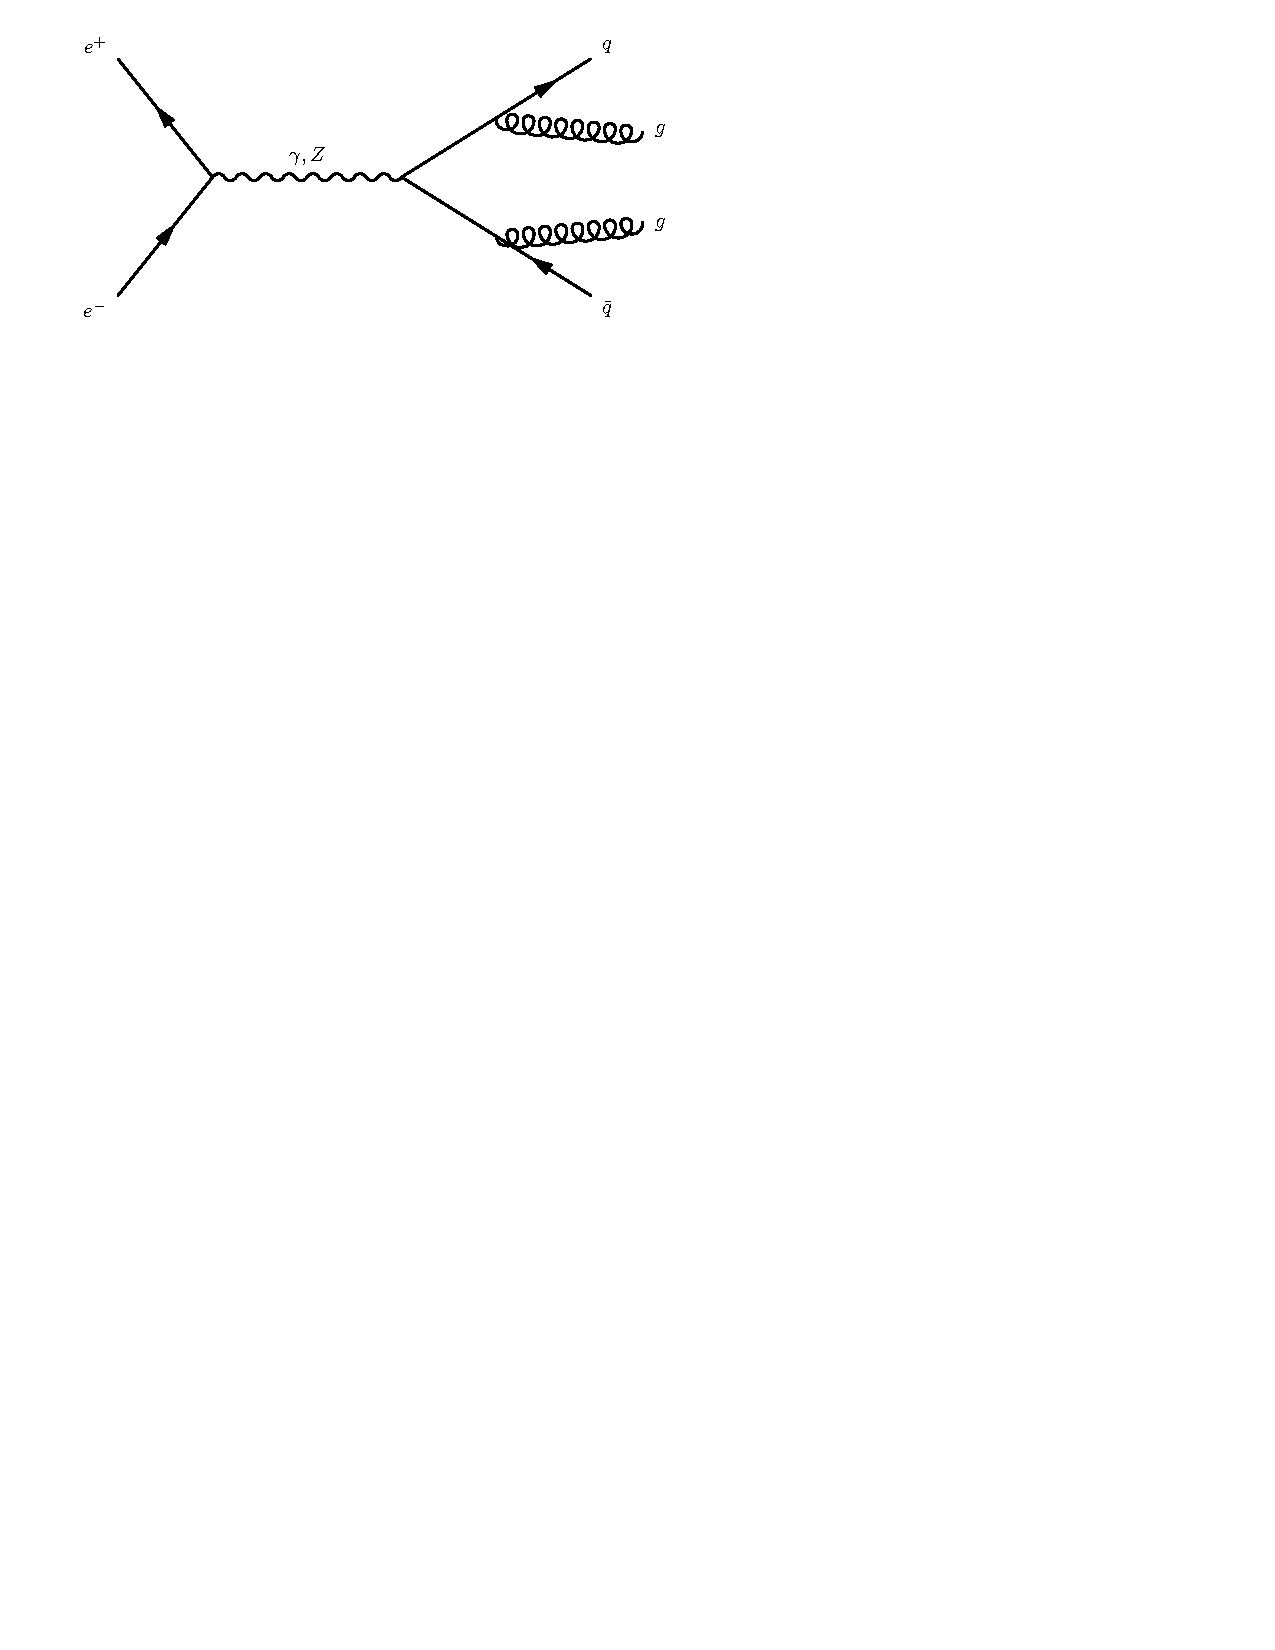
\includegraphics[trim={0.5cm 22cm 10cm 0cm},width=\textwidth]{../Diagrams/D1.pdf}
    \caption{$e^+e^- \rightarrow q\bar{q}gg$ (EM/WI, SI)}
    \label{fey:1}
  \end{subfigure}%
  ~
  \begin{subfigure}[b]{0.3\textwidth}
    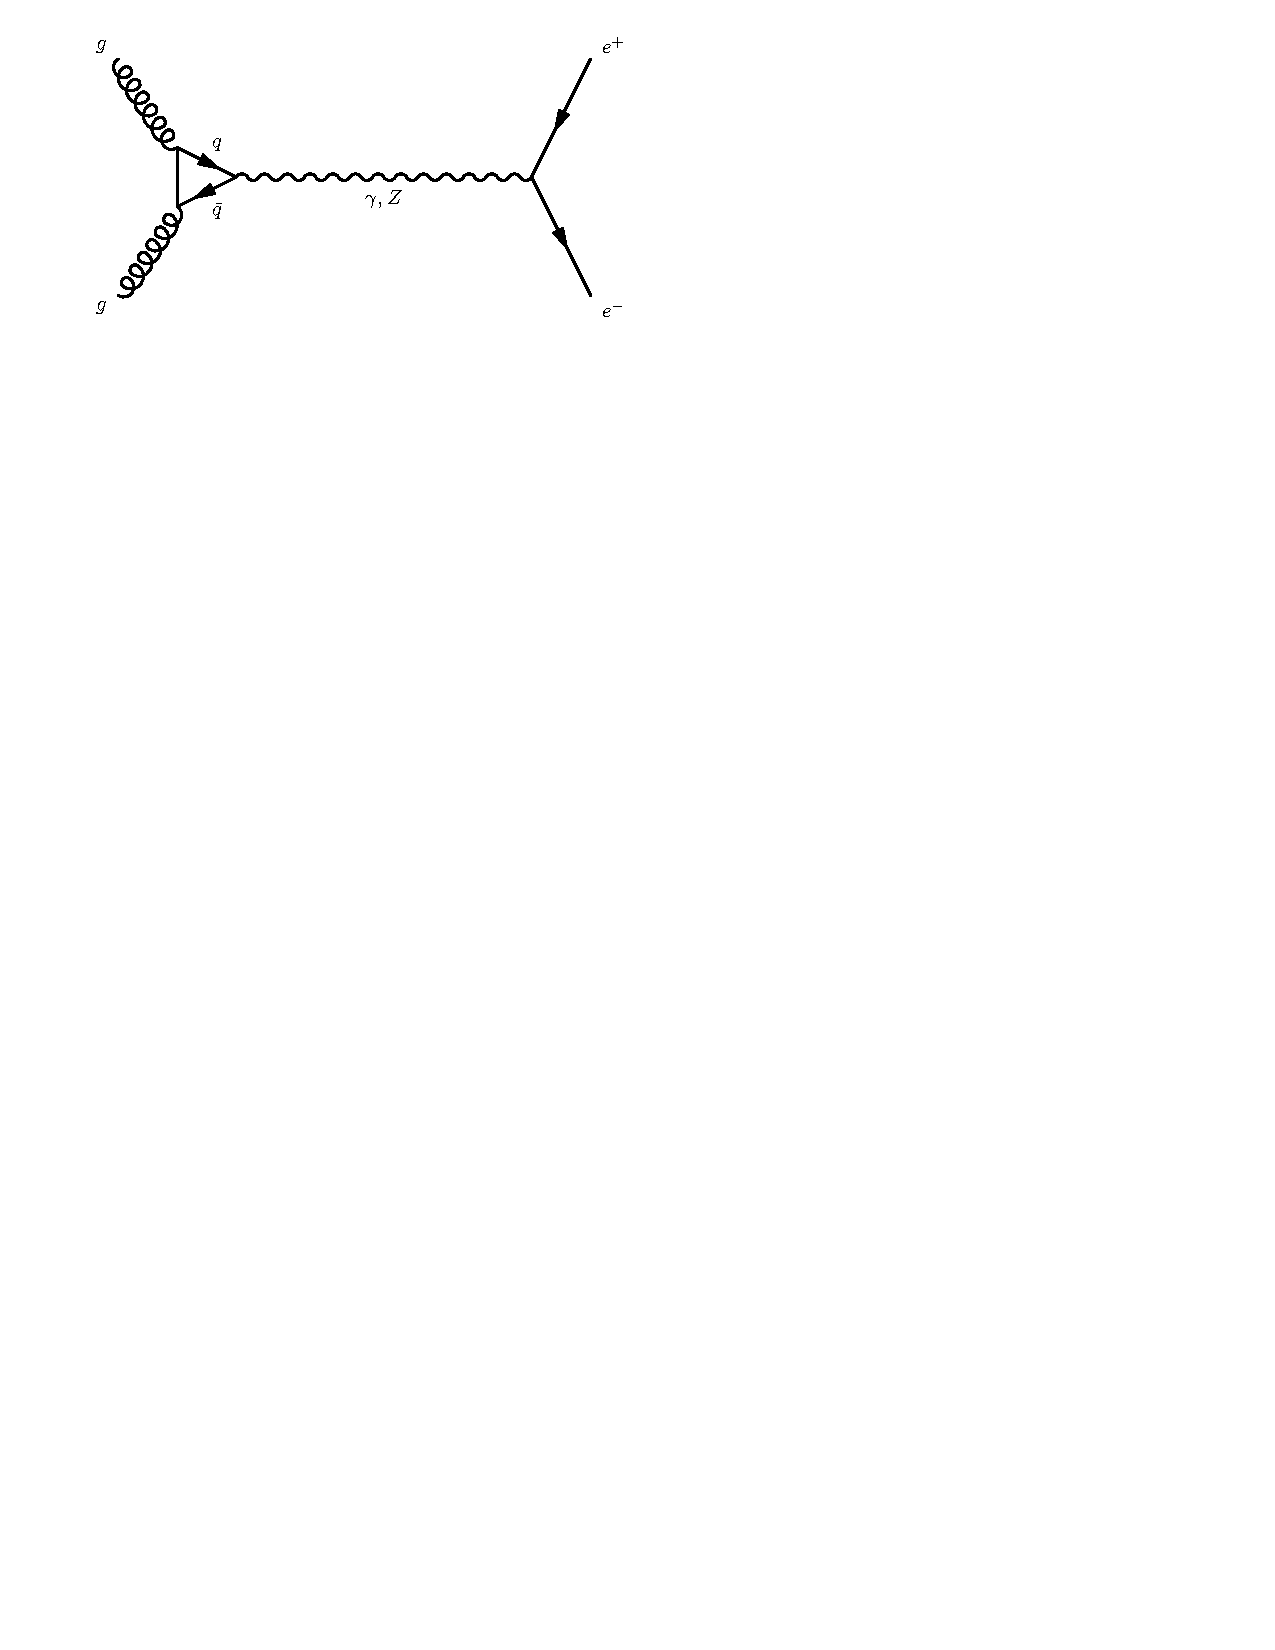
\includegraphics[trim={0.5cm 22cm 10cm 0cm},width=\textwidth]{../Diagrams/D2.pdf}
    \caption{$gg\rightarrow e^+e^-$ (SI, EM/WI)}
    \label{fey:2}
  \end{subfigure}%
  ~
  \begin{subfigure}[b]{0.3\textwidth}
    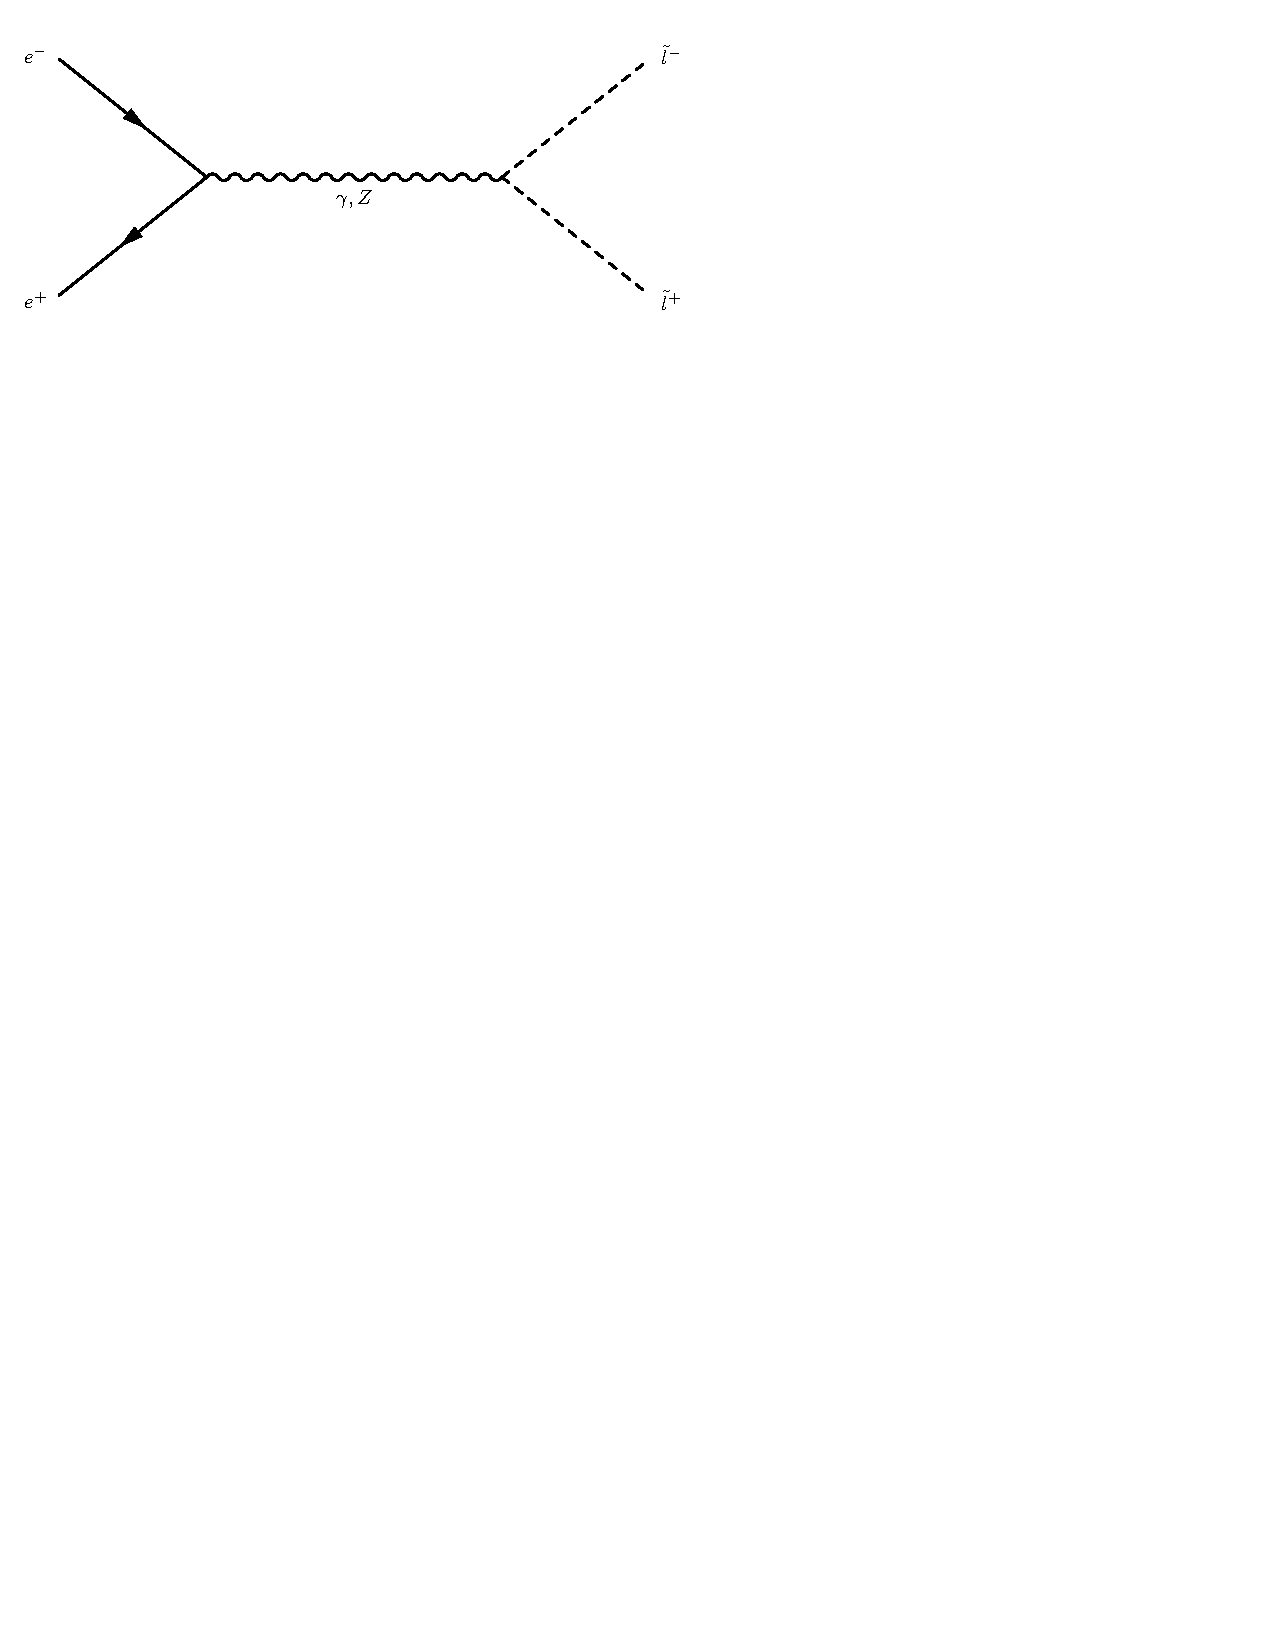
\includegraphics[trim={0.5cm 22cm 10cm 0cm},width=\textwidth]{../Diagrams/D3.pdf}
    \caption{$e^+e^-\rightarrow \tilde{l}^+\tilde{l}^-$ (EM/WI)}
    \label{fey:3}
  \end{subfigure}
  \newline
  \newline
  \begin{subfigure}[b]{0.3\textwidth}
    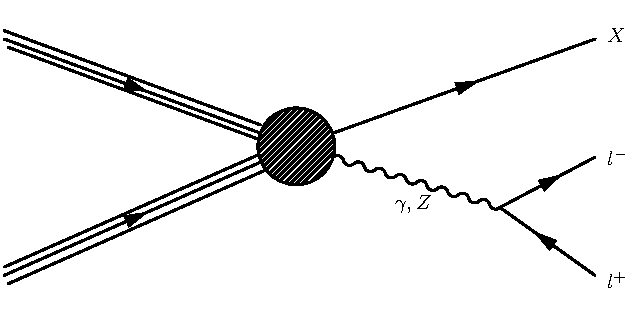
\includegraphics[trim={0.5cm 22cm 10cm 0cm},width=\textwidth]{../Diagrams/D4.pdf}
    \caption{$p\bar{p}\rightarrow l^+l^-X$ (any)}
    \label{fey:4}
  \end{subfigure}%
  ~
  \begin{subfigure}[b]{0.3\textwidth}
    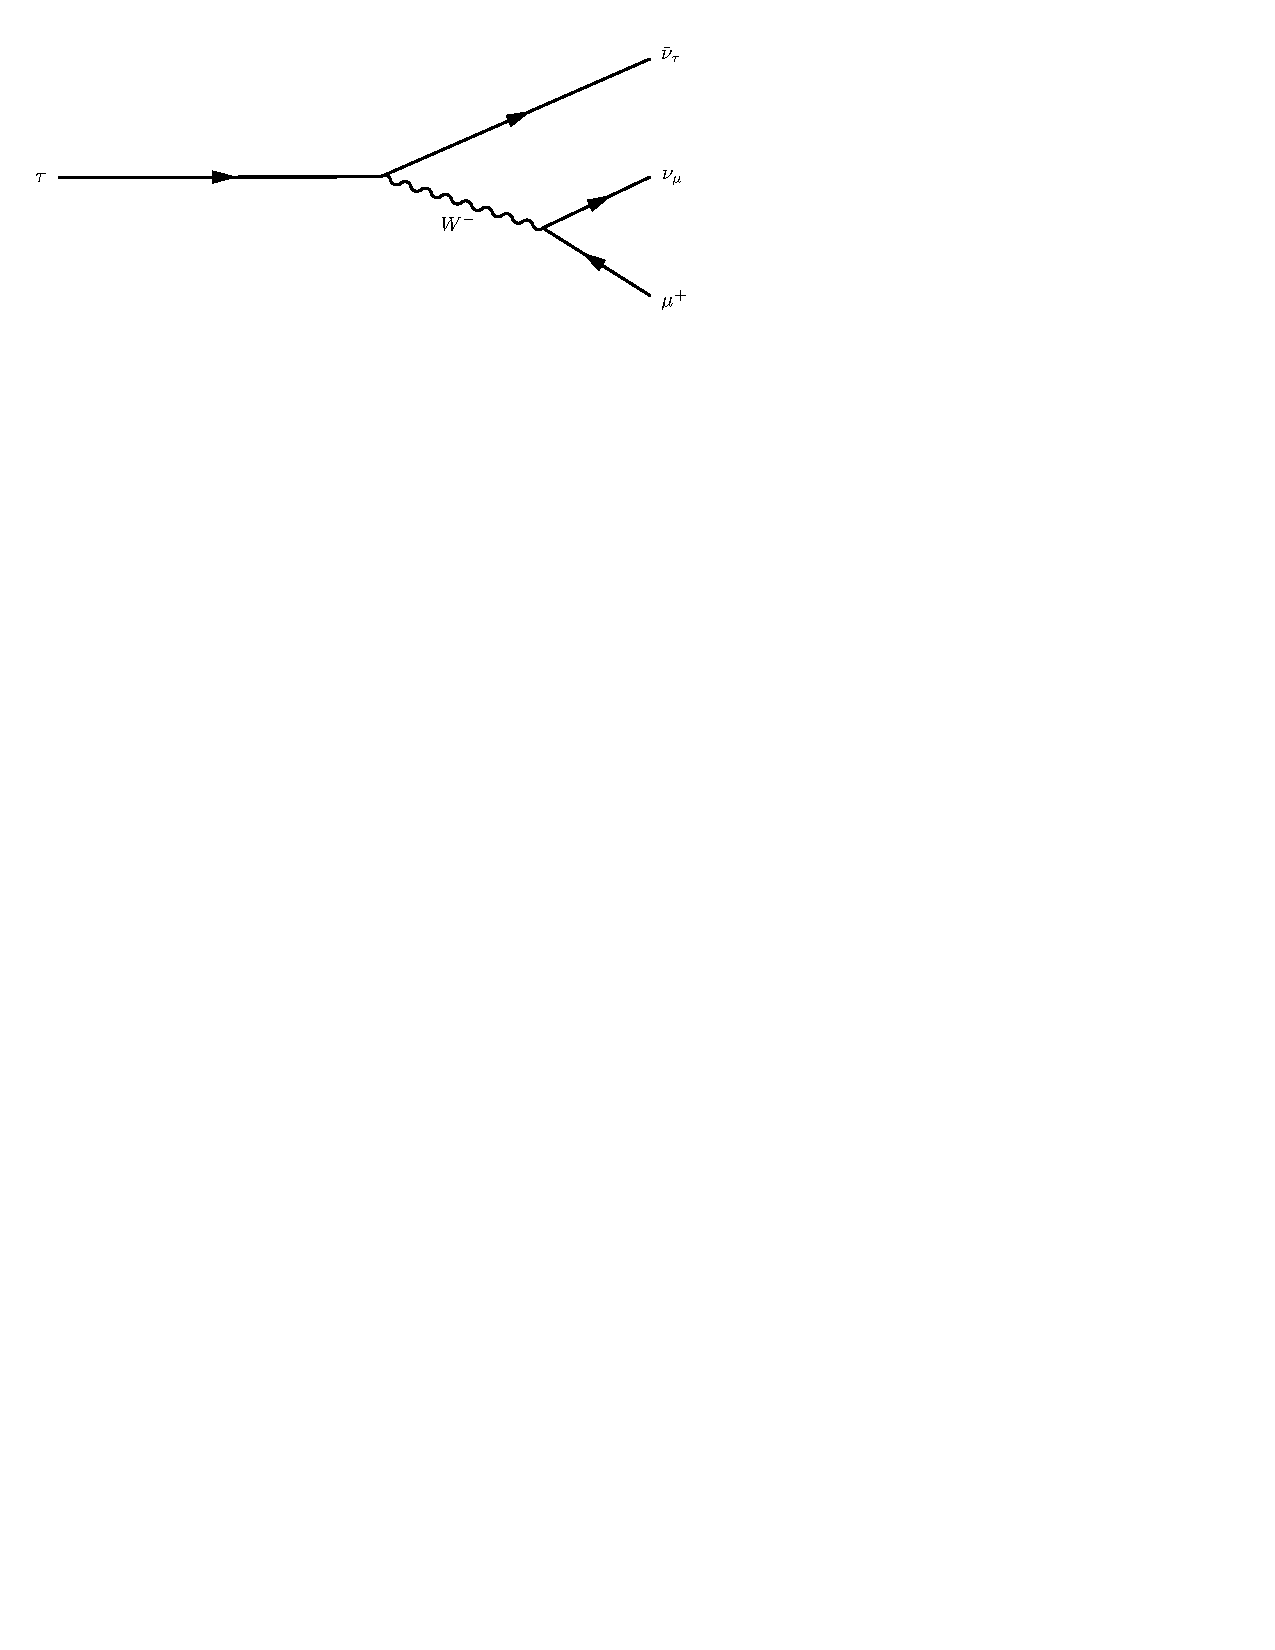
\includegraphics[trim={0.5cm 22cm 10cm 0cm},width=\textwidth]{../Diagrams/D5.pdf}
    \caption{$\tau^+\rightarrow \mu^+\bar{\nu}_{\tau}\nu_{e/\mu}$ (WI)}
    \label{fey:5}
  \end{subfigure}%
  ~
  \begin{subfigure}[b]{0.3\textwidth}
    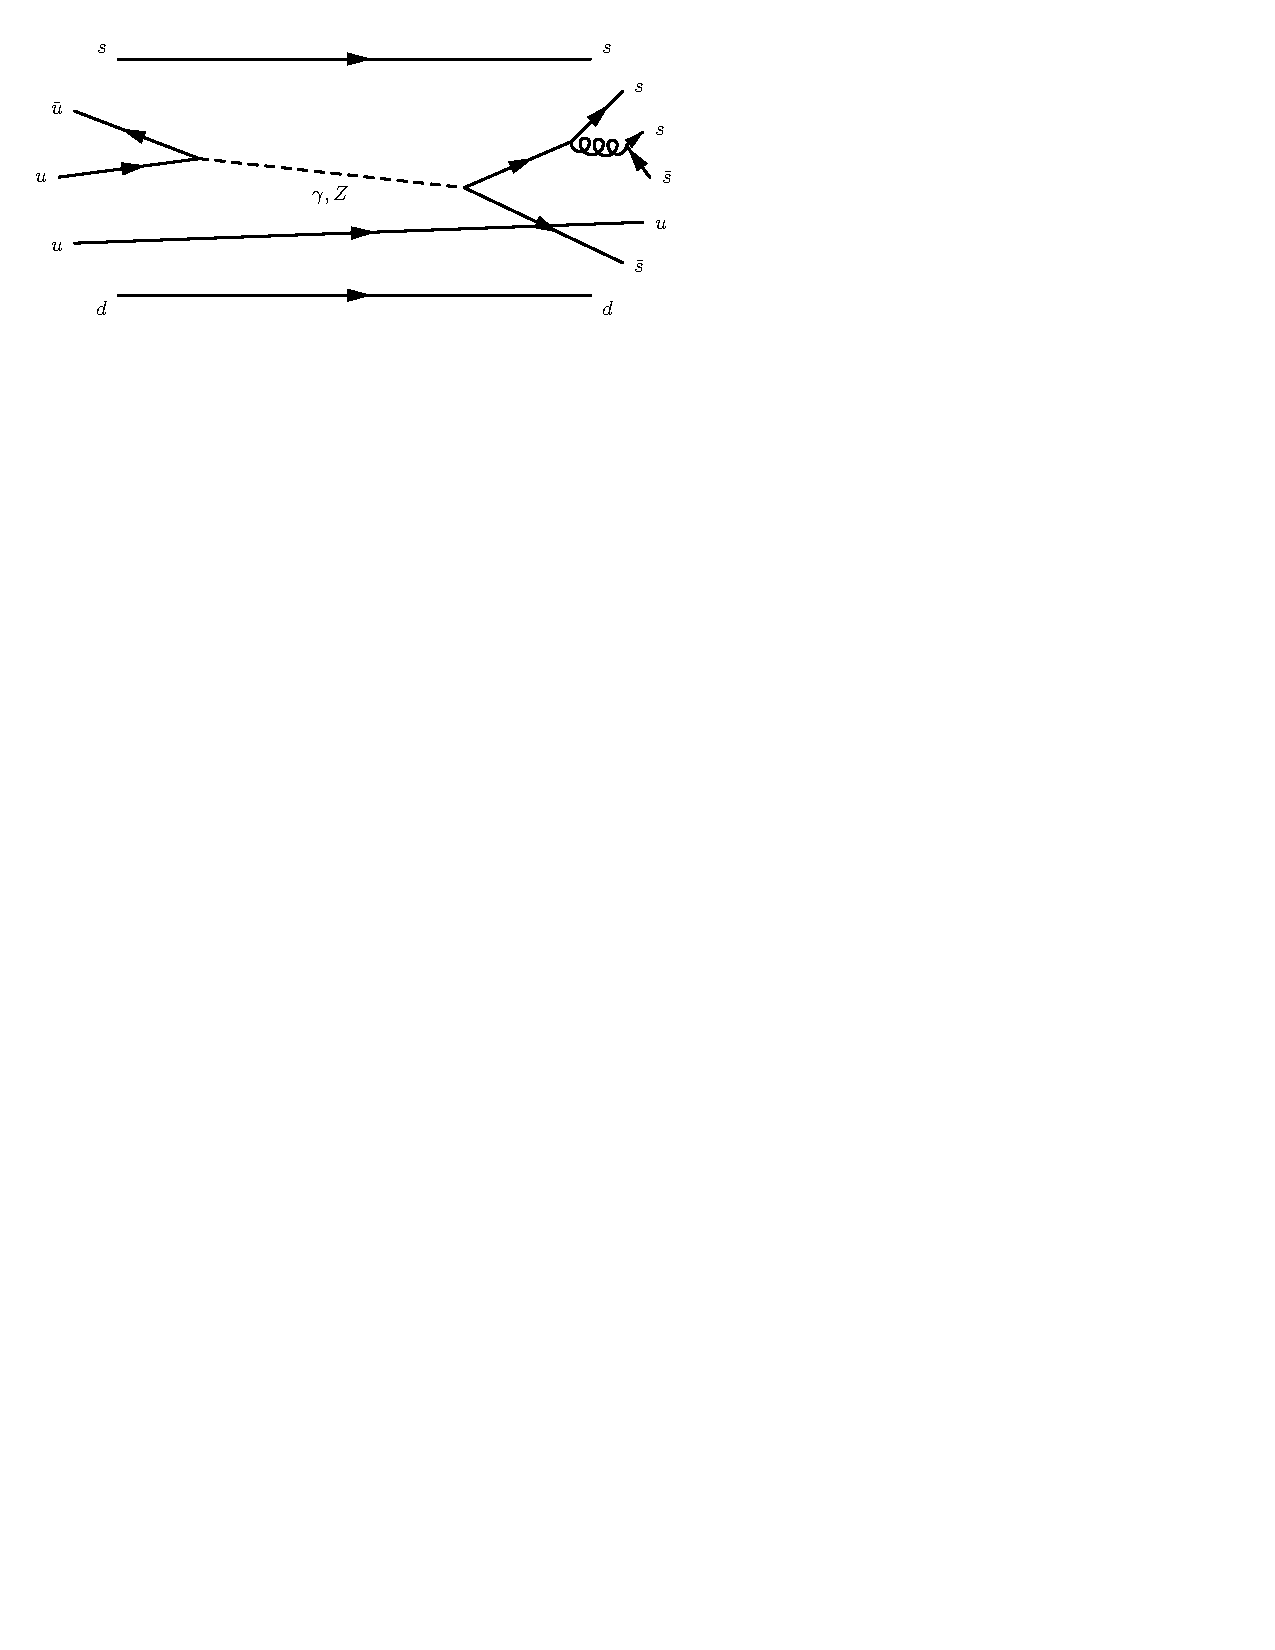
\includegraphics[trim={0.5cm 22cm 10cm 0cm},width=\textwidth]{../Diagrams/D6.pdf}
    \caption{$K^-p \rightarrow \Omega^-K^+K^0$ (EM/WI, SI)}
    \label{fey:6}
  \end{subfigure}
  \newline
  \newline
  \begin{subfigure}[b]{0.3\textwidth}
    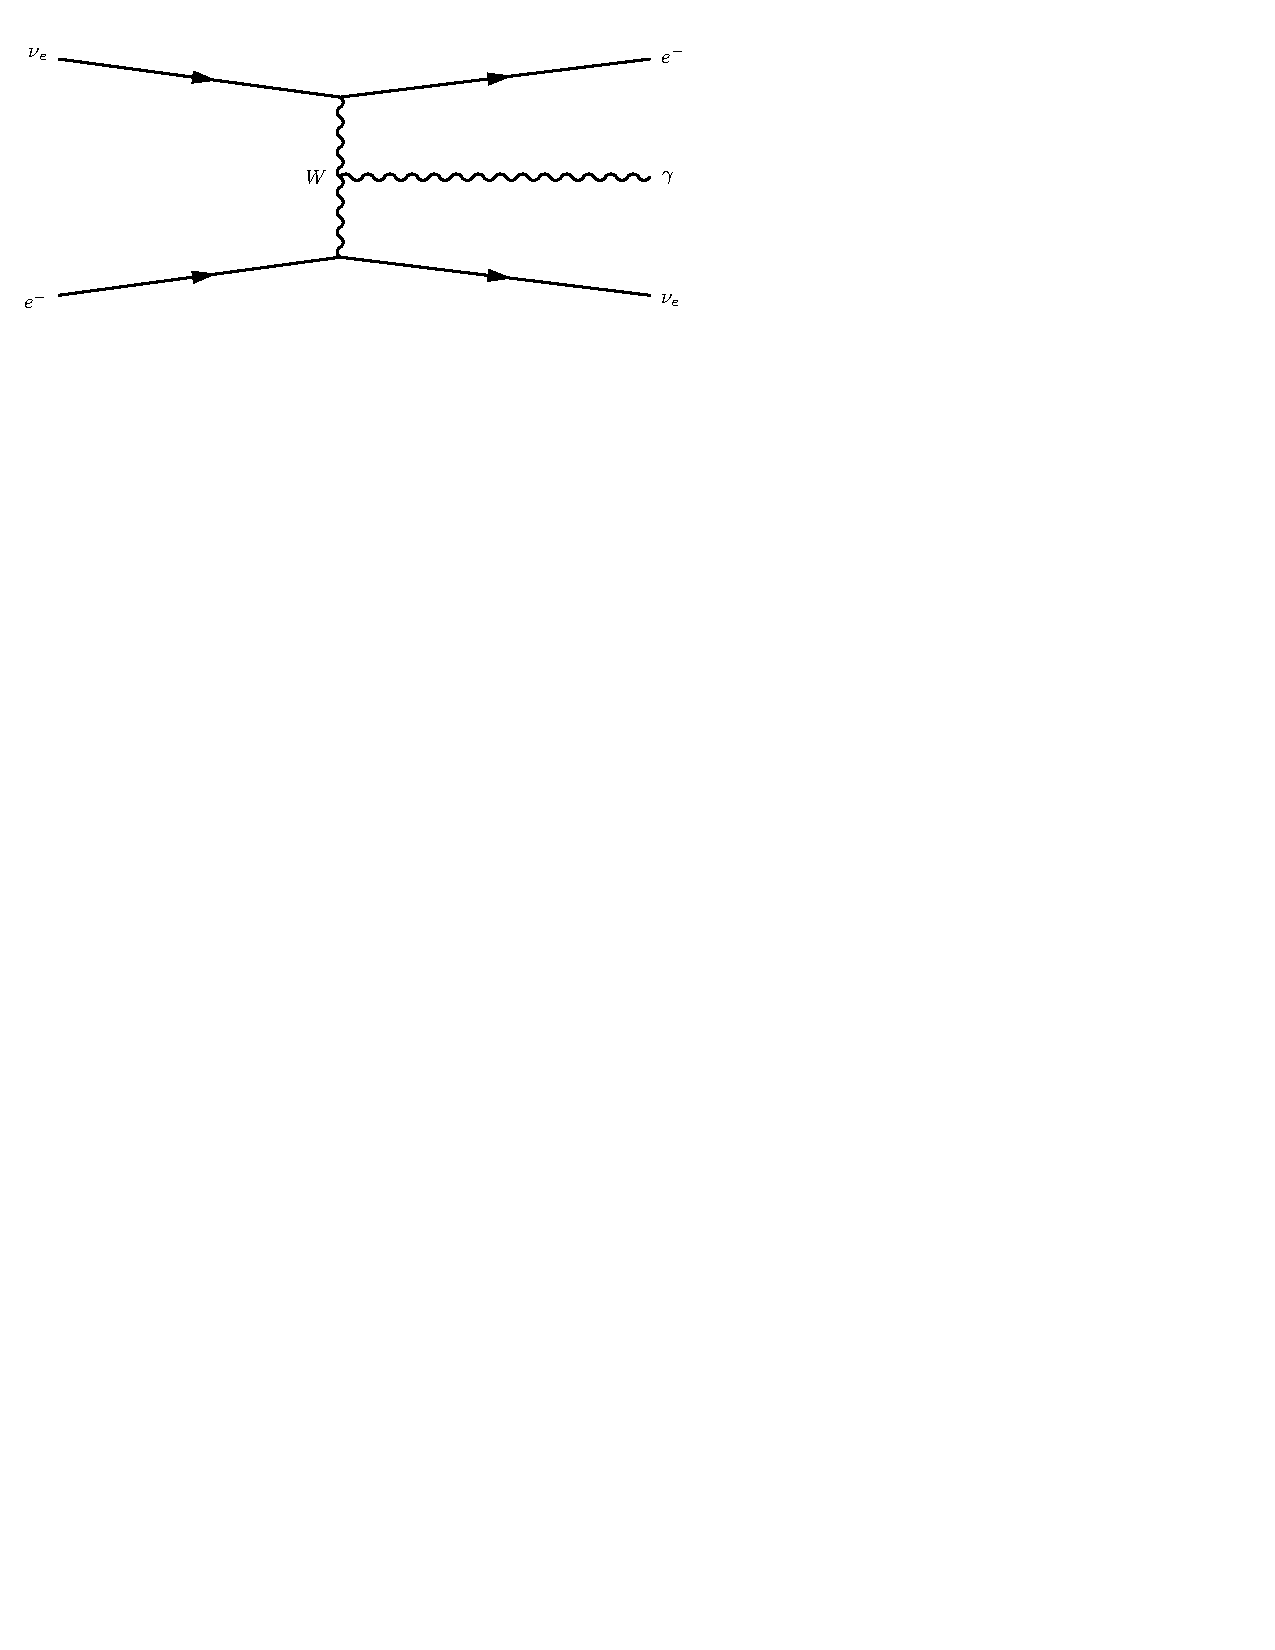
\includegraphics[trim={0.5cm 22cm 10cm 0cm},width=\textwidth]{../Diagrams/D7.pdf}
    \caption{$e^-\nu_e\rightarrow \nu_e \gamma e^-$ (WI,EM)}
    \label{fey:7}
  \end{subfigure}%
  ~
  \begin{subfigure}[b]{0.3\textwidth}
    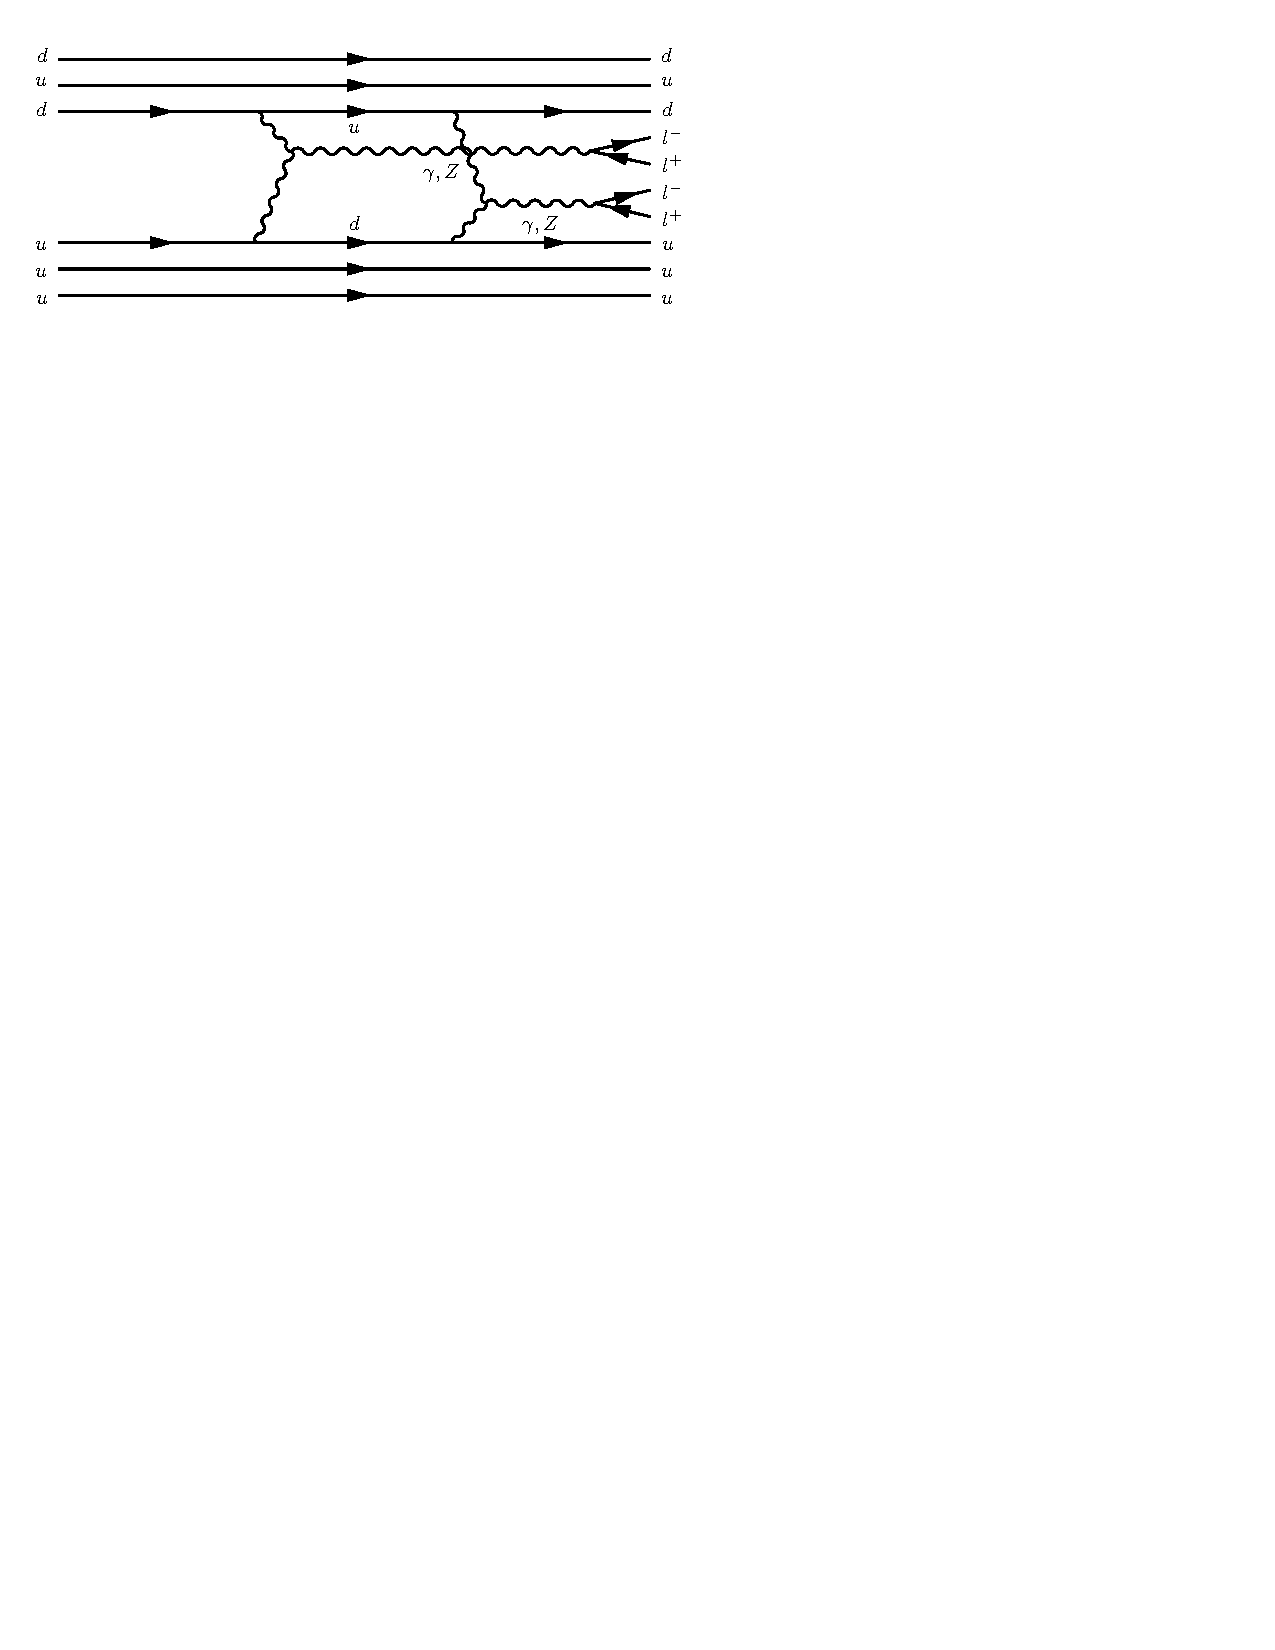
\includegraphics[trim={0.5cm 22cm 10cm 0cm},width=\textwidth]{../Diagrams/D8.pdf}
    \caption{$pp\rightarrow ppl^+l^-l^+l^-$ (WI, (EM))}
    \label{fey:8}
  \end{subfigure}%
  ~
  \begin{subfigure}[b]{0.3\textwidth}
    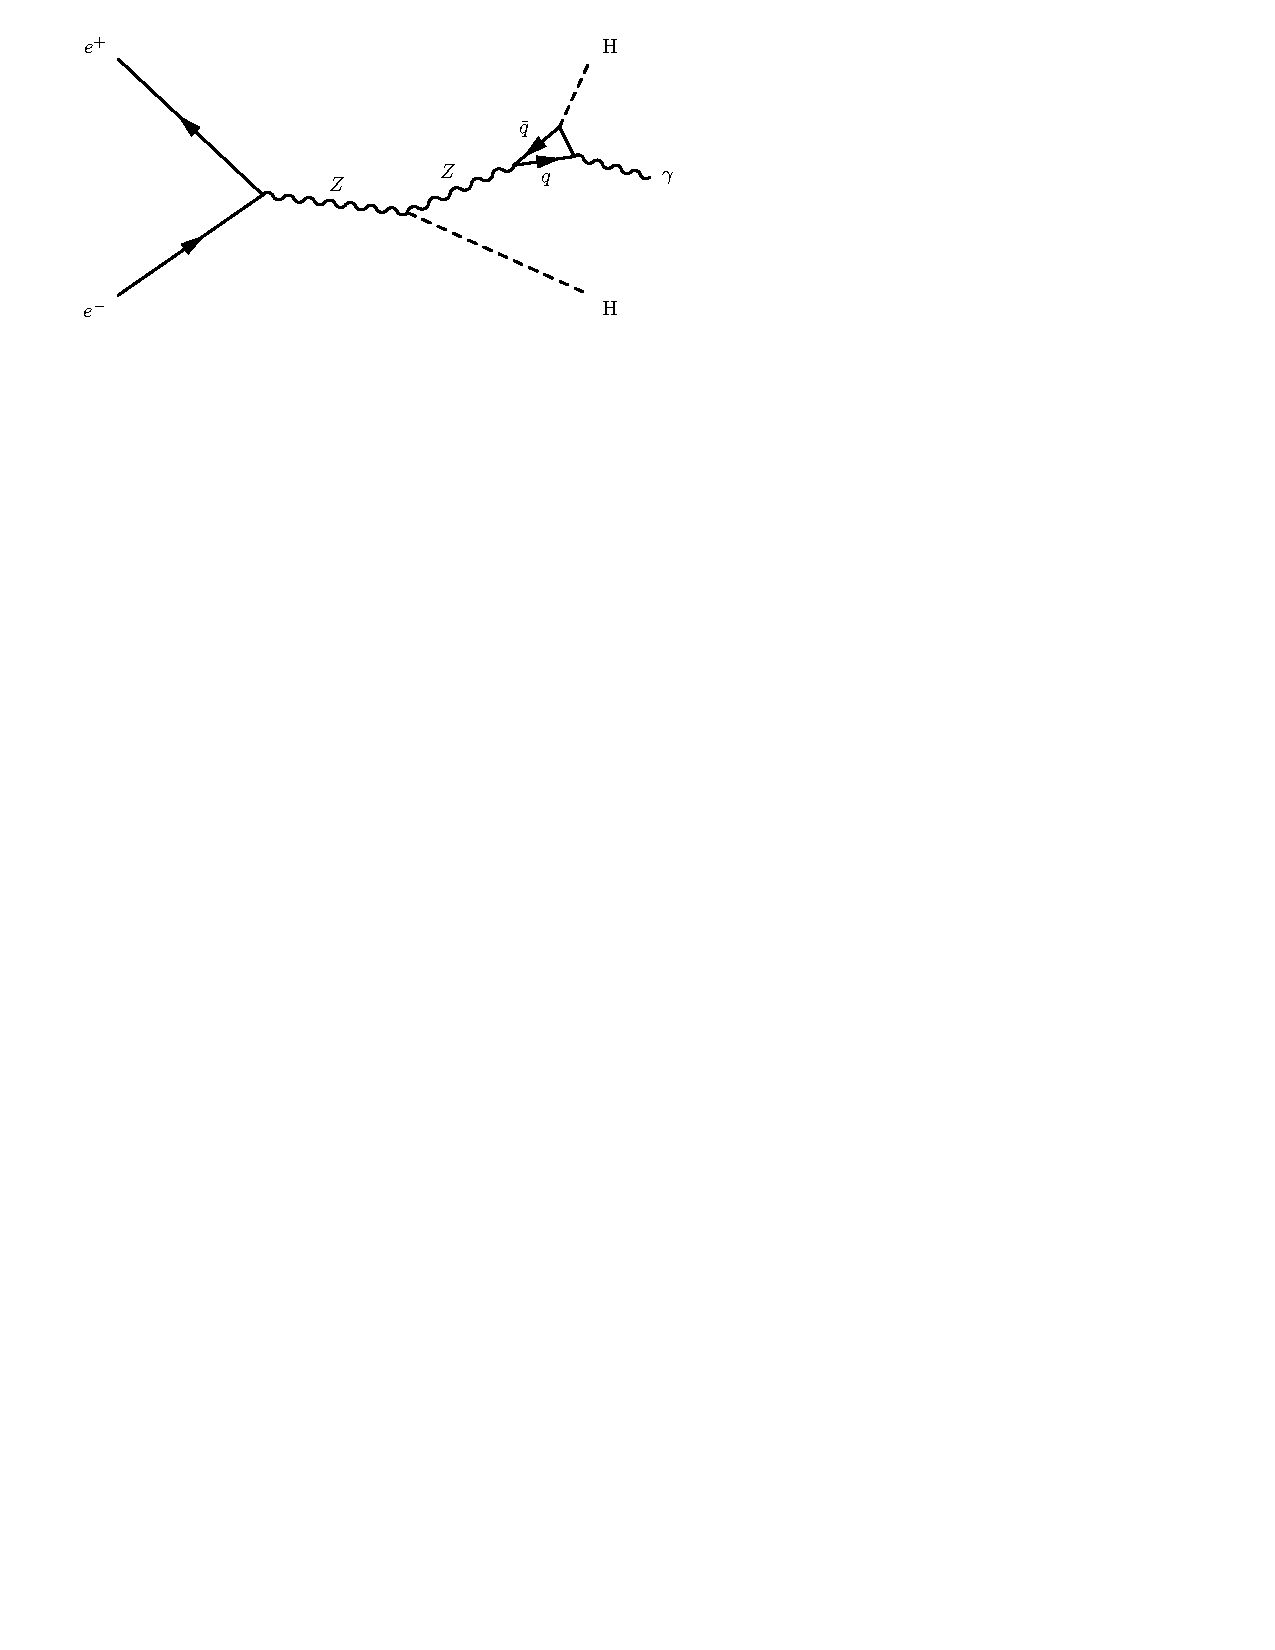
\includegraphics[trim={0.5cm 22cm 10cm 0cm},width=\textwidth]{../Diagrams/D9.pdf}
    \caption{$e^-e^+ \rightarrow \gamma HH$ (WI, EM)}
    \label{fey:9}
  \end{subfigure}
  \newline
  \newline
  \begin{subfigure}[b]{0.3\textwidth}
    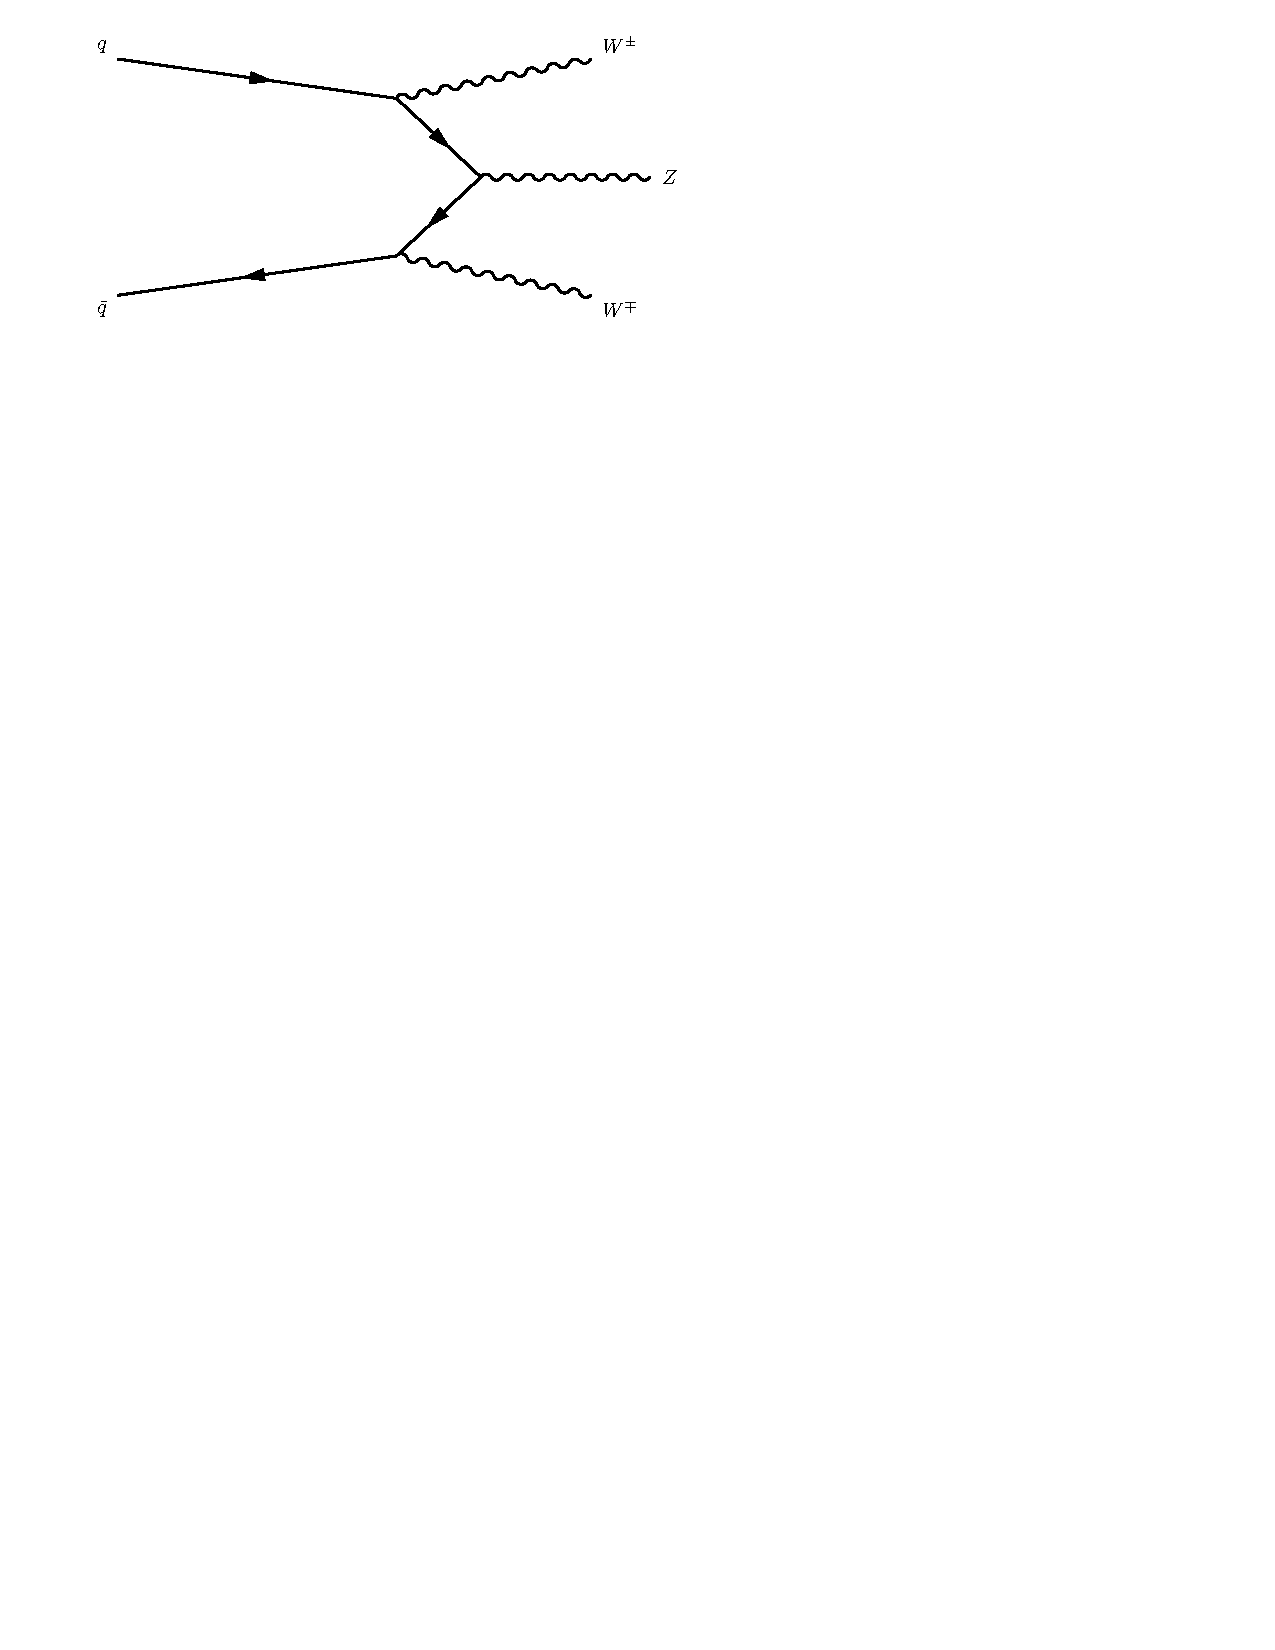
\includegraphics[trim={0.5cm 22cm 10cm 0cm},width=\textwidth]{../Diagrams/D10.pdf}
    \caption{$qq\rightarrow W^{+}W^{-}Z$ (WI)}
    \label{fey:10}
  \end{subfigure}%
  ~
  \begin{subfigure}[b]{0.3\textwidth}
    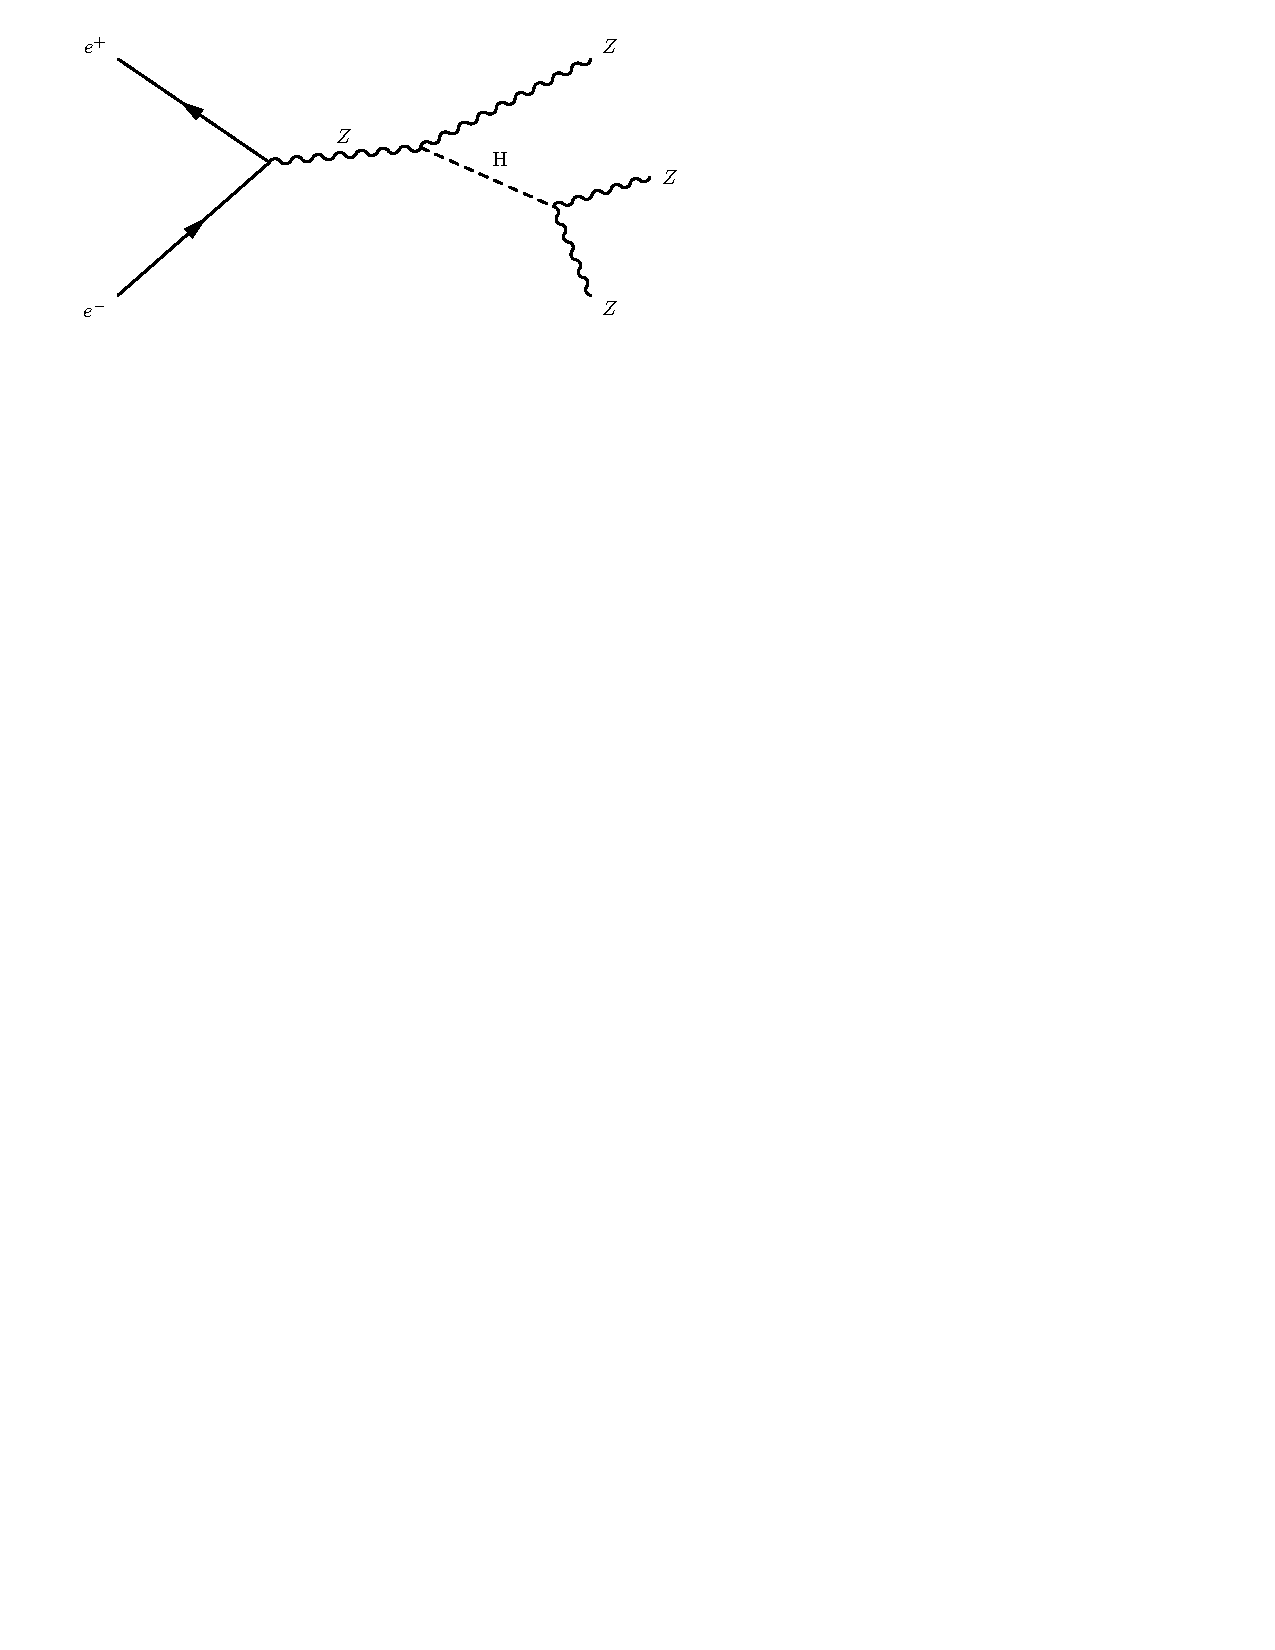
\includegraphics[trim={0.5cm 22cm 10cm 0cm},width=\textwidth]{../Diagrams/D11.pdf}
    \caption{$e^-e^+\rightarrow ZZ$ (WI)}
    \label{fey:11}
  \end{subfigure}%
  ~
  \begin{subfigure}[b]{0.3\textwidth}
    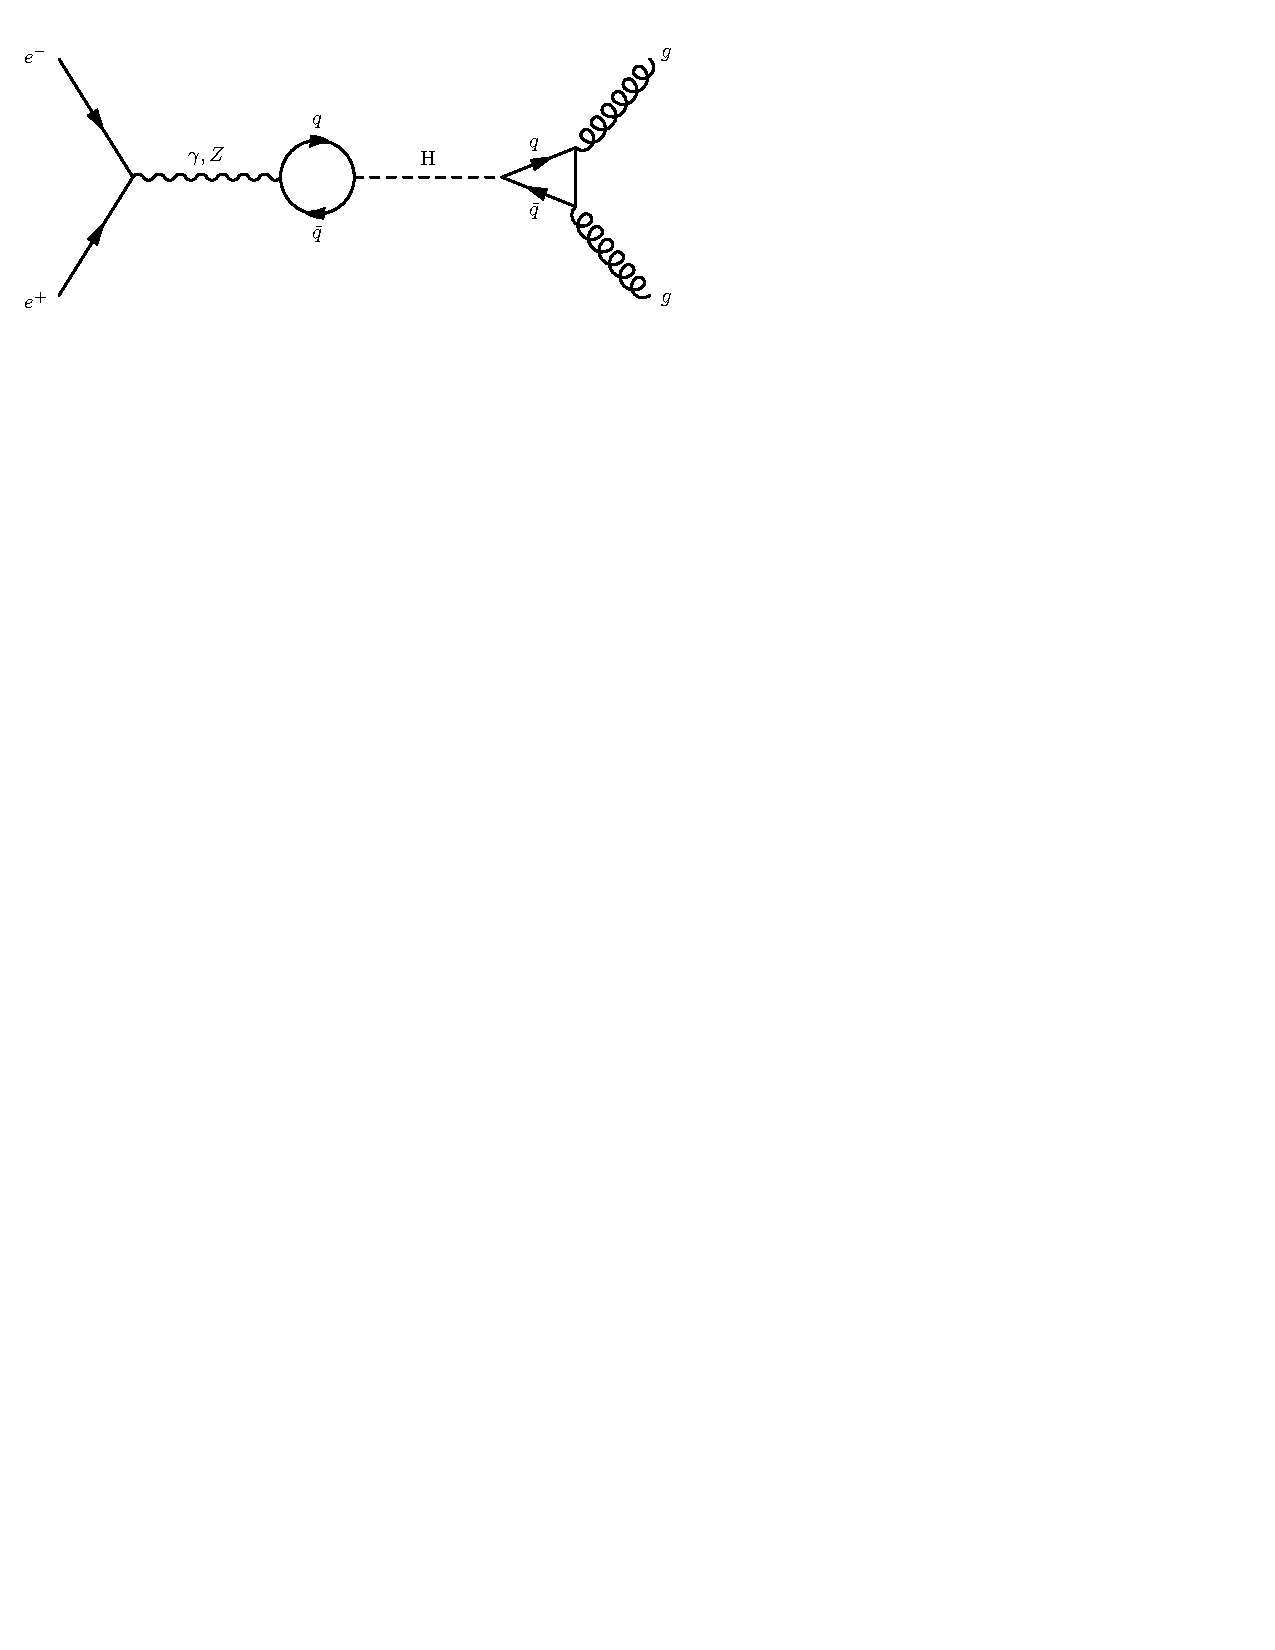
\includegraphics[trim={0.5cm 22cm 10cm 0cm},width=\textwidth]{../Diagrams/D12.pdf}
    \caption{$e^-e^+\rightarrow H \rightarrow gg$ (Electroweak, SI)}
    \label{fey:12}
  \end{subfigure}
  \newline
  \newline
  \begin{subfigure}[b]{0.3\textwidth}
    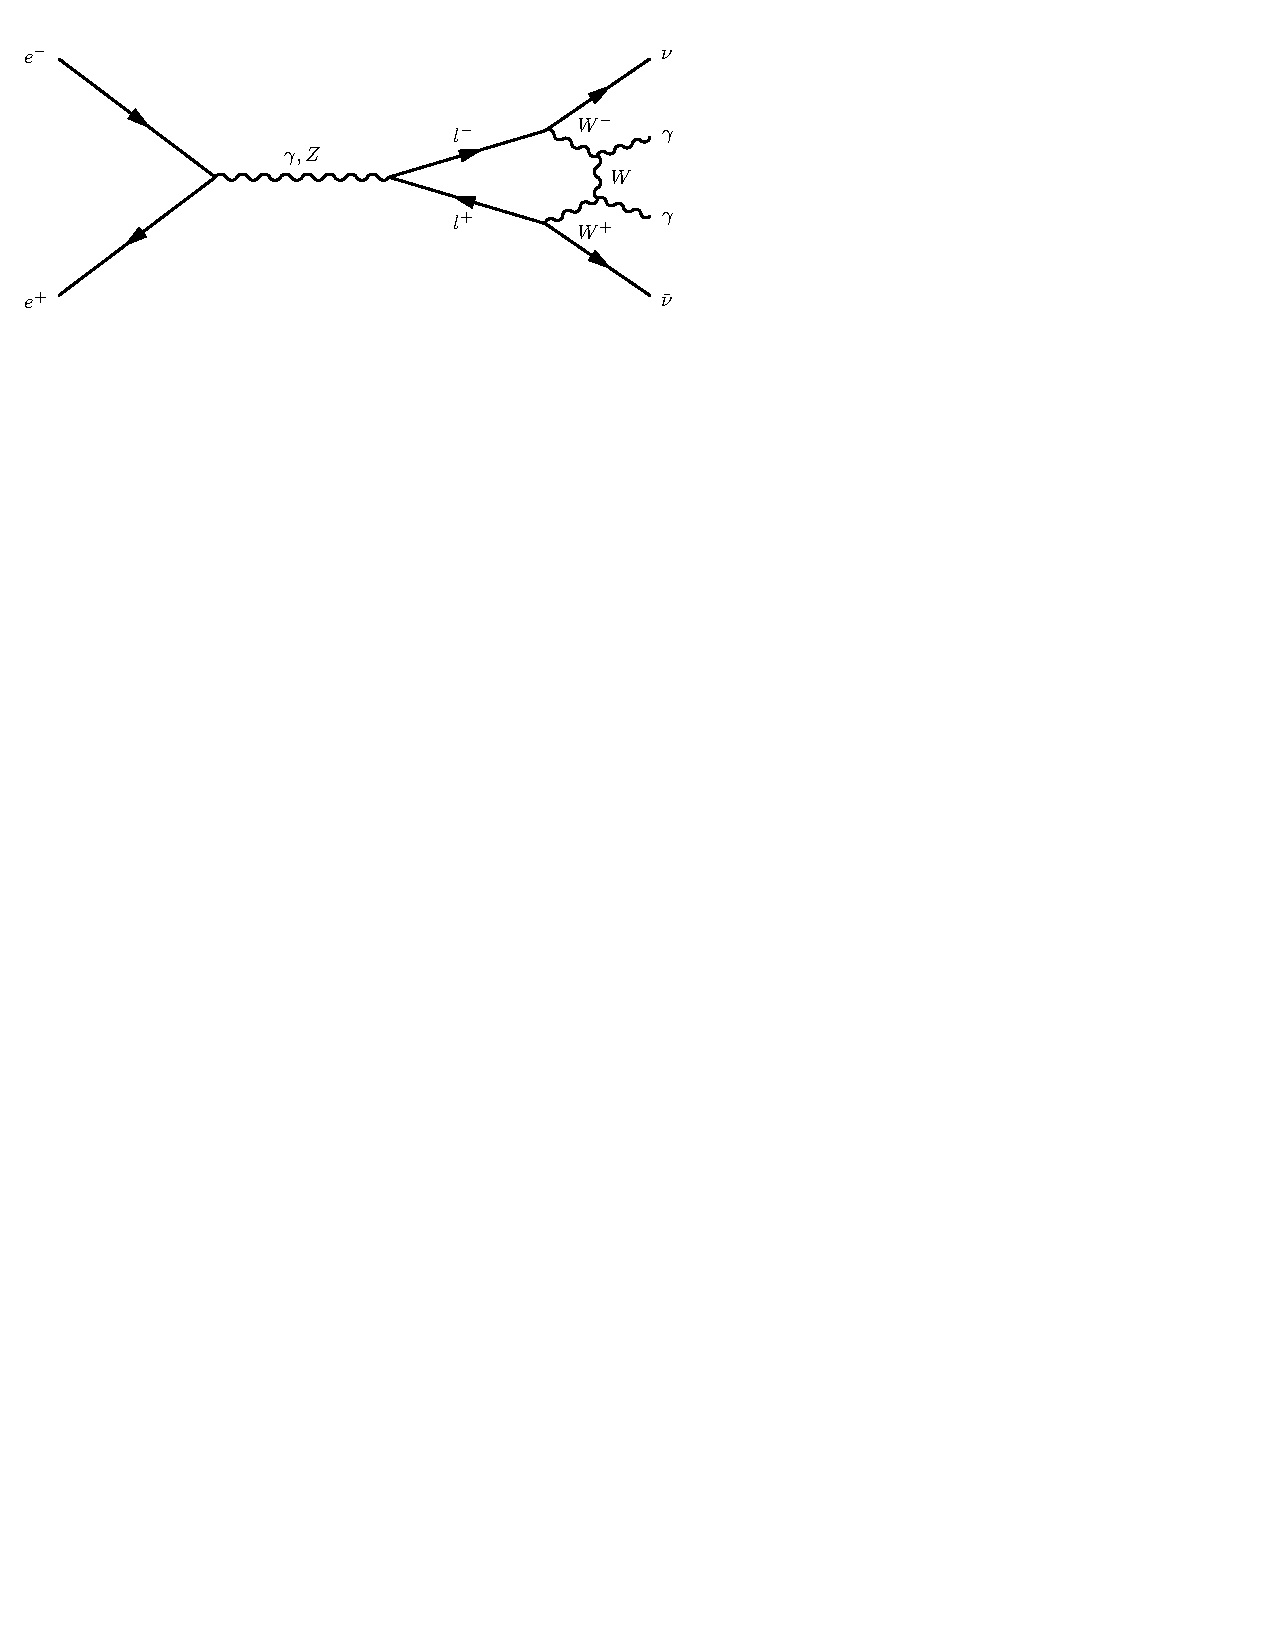
\includegraphics[trim={0.5cm 22cm 10cm 0cm},width=\textwidth]{../Diagrams/D13.pdf}
    \caption{$e^+e^- \rightarrow \nu\bar{\nu}\gamma\gamma$ (WI, EM)}
    \label{fey:13}
  \end{subfigure}%
  ~
  \begin{subfigure}[b]{0.3\textwidth}
    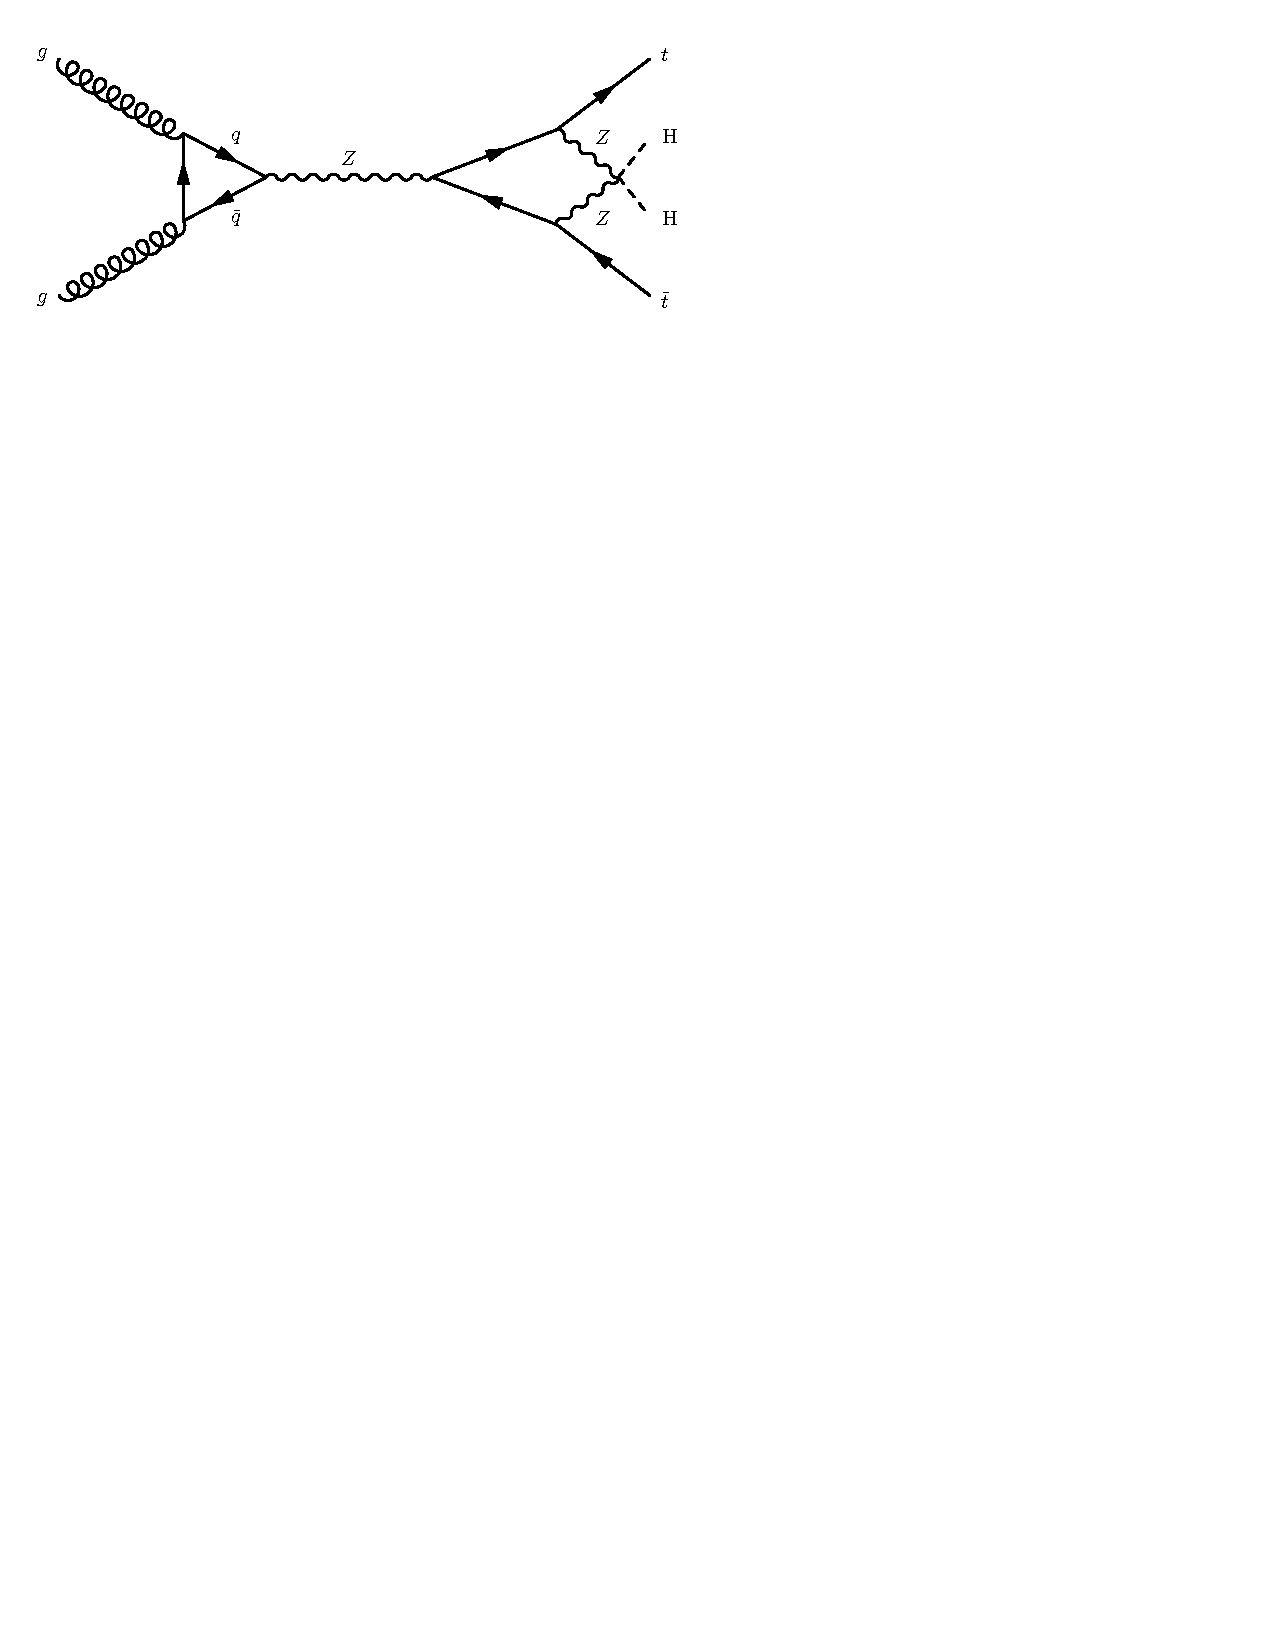
\includegraphics[trim={0.5cm 22cm 10cm 0cm},width=\textwidth]{../Diagrams/D14.pdf}
    \caption{$gg\rightarrow t\bar{t}HH$ (SI, WI, (EM))}
    \label{fey:14}
  \end{subfigure}%
  ~
  \begin{subfigure}[b]{0.3\textwidth}
    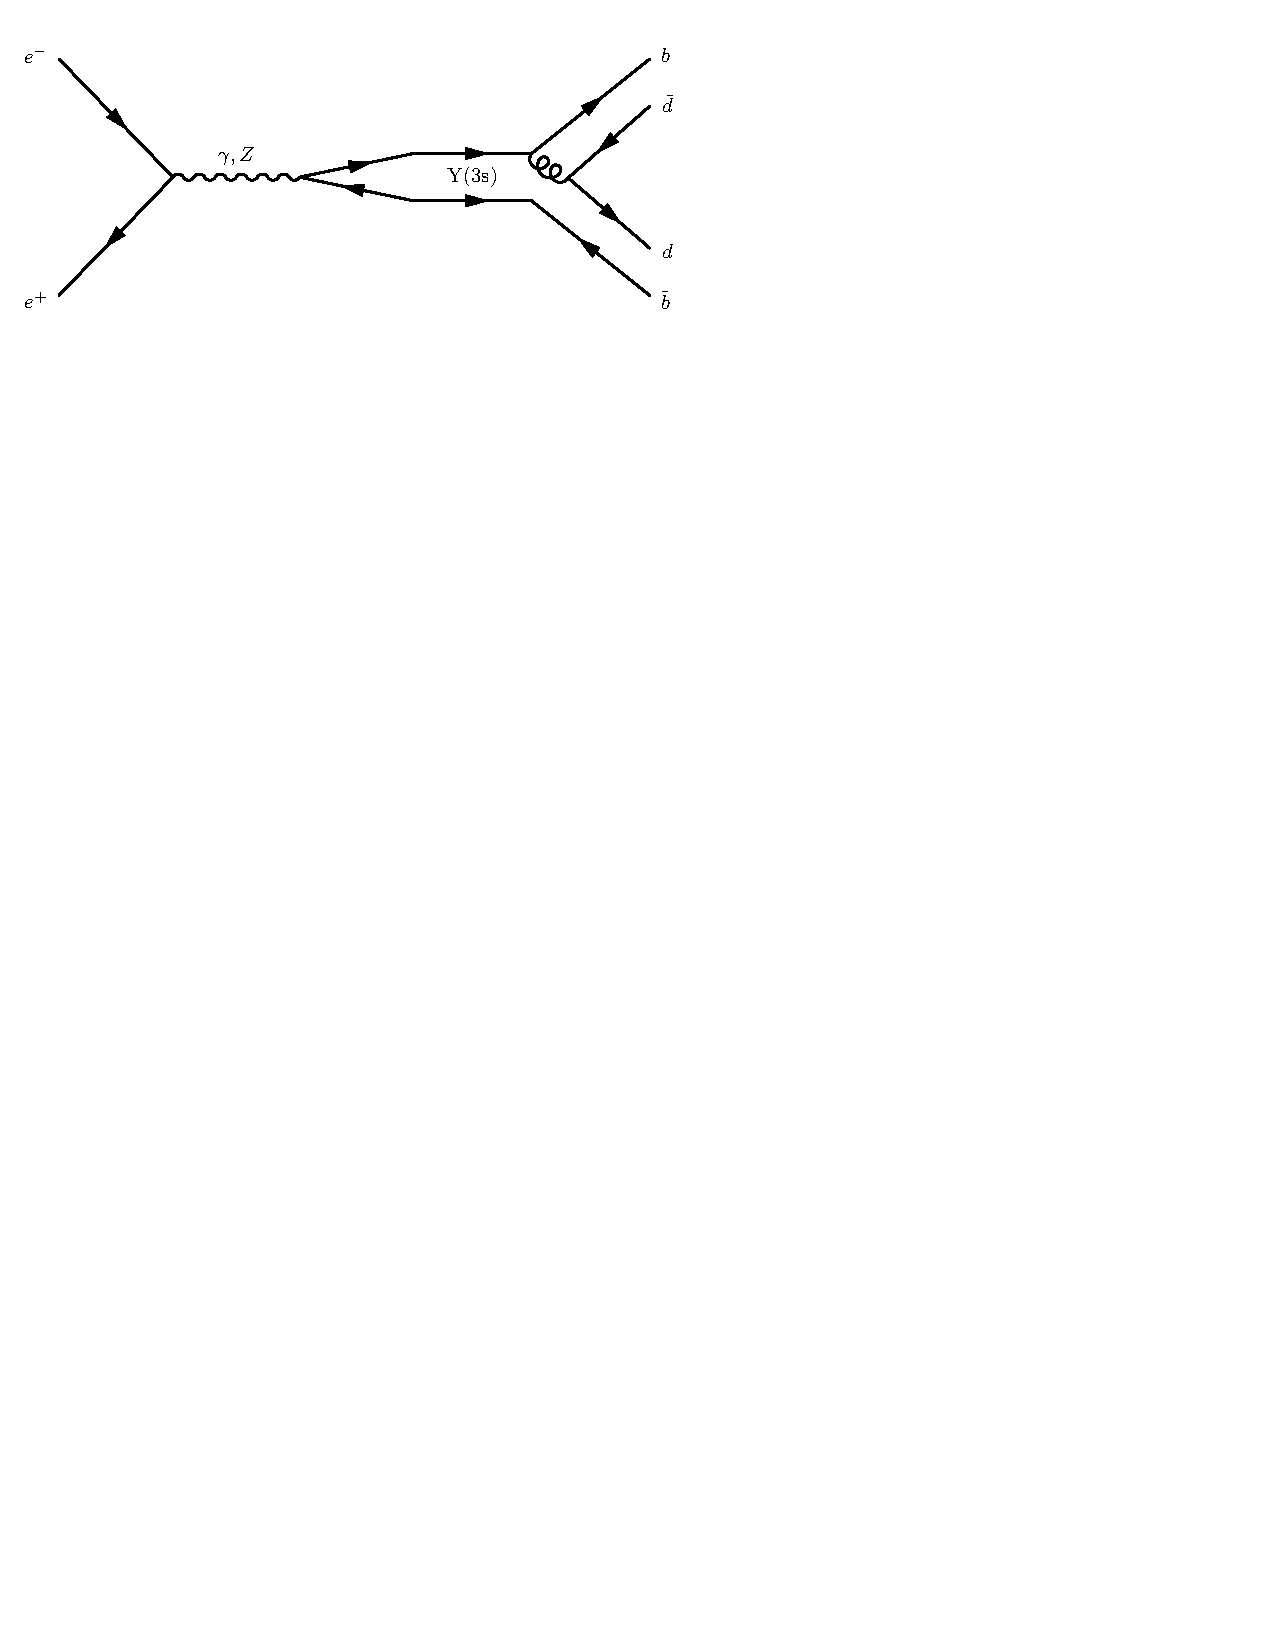
\includegraphics[trim={0.5cm 22cm 10cm 0cm},width=\textwidth]{../Diagrams/D15.pdf}
    \caption{$e^+e^-\rightarrow \Upsilon(3s)\rightarrow B^0\bar{B^0}$ (WI/EM, SI)}
    \label{fey:15}
  \end{subfigure}
  \newline
  \newline
  \begin{subfigure}[b]{0.3\textwidth}
    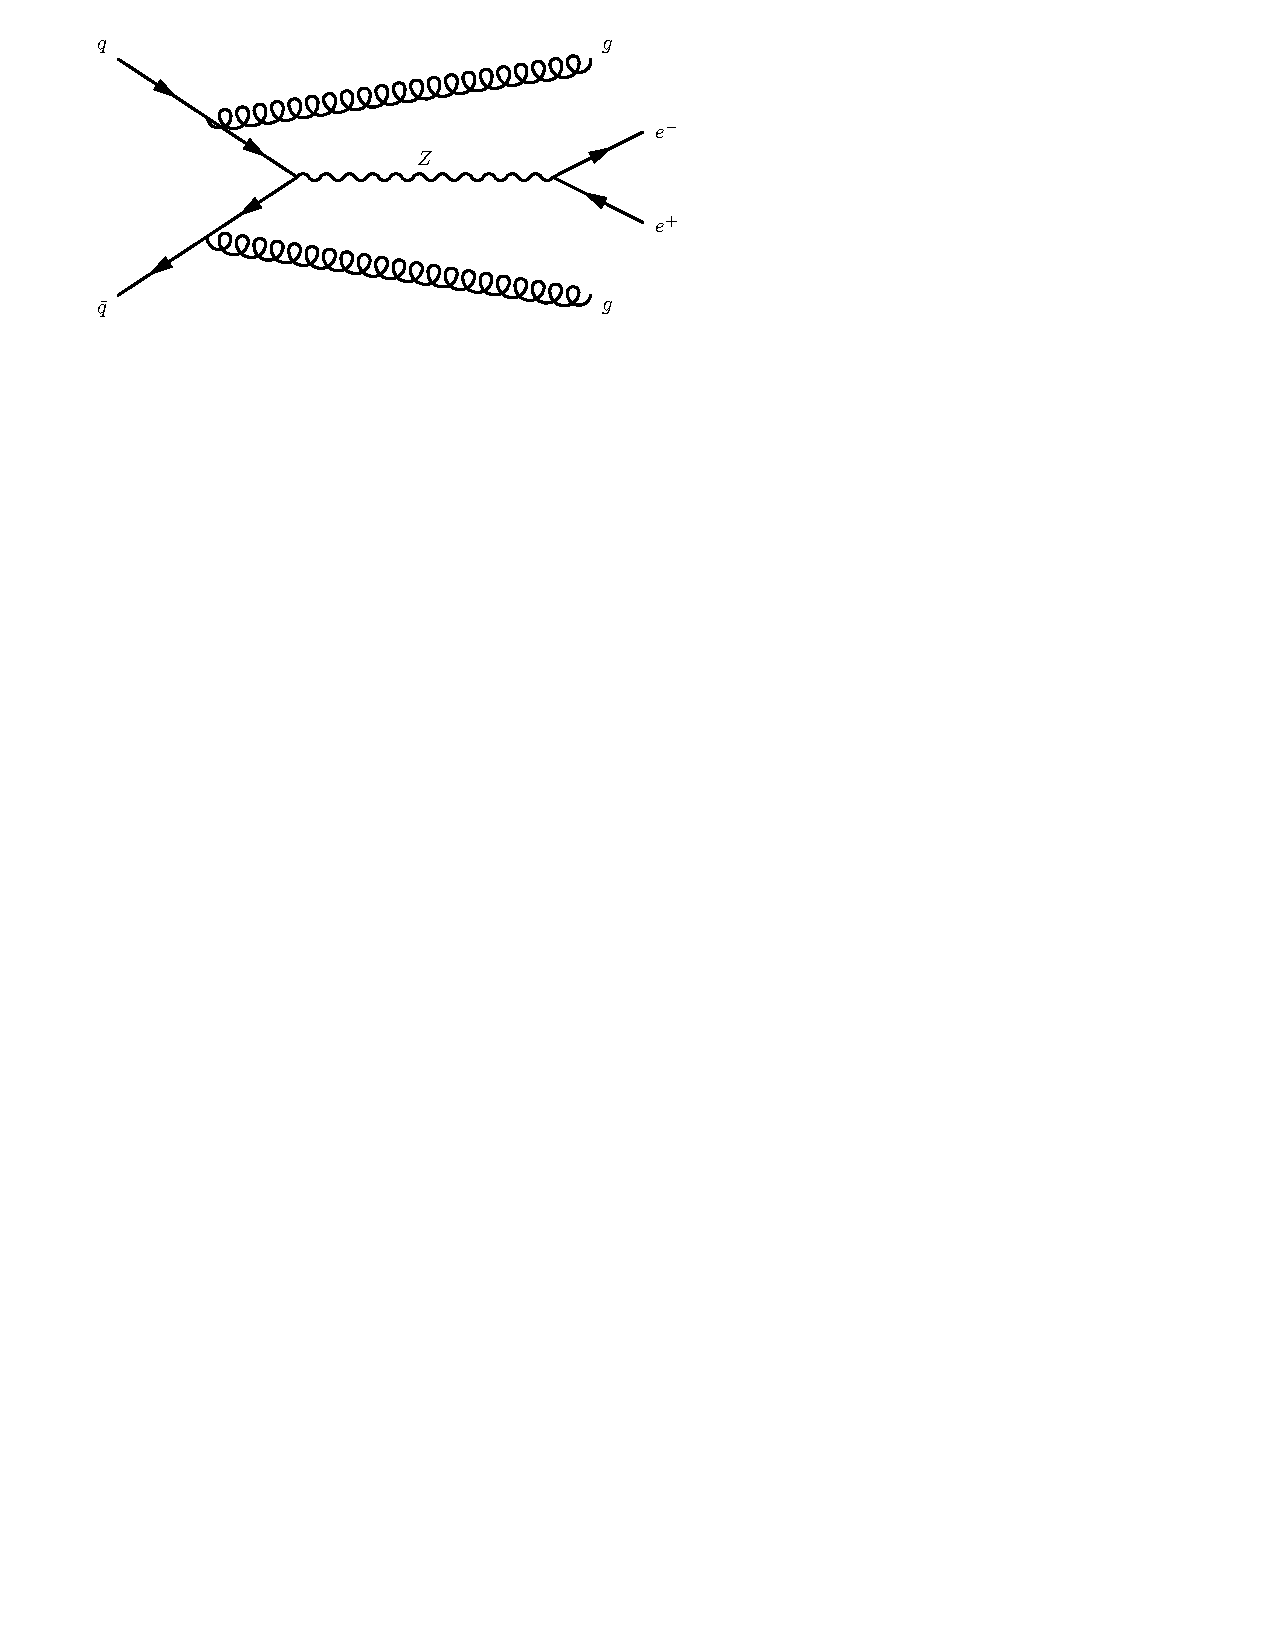
\includegraphics[trim={0.5cm 22cm 10cm 0cm},width=\textwidth]{../Diagrams/D16.pdf}
    \caption{$q\bar{q}\rightarrow gge^-e^+$ (SI, WI/EM)}
    \label{fey:16}
  \end{subfigure}
  ~
  \begin{subfigure}[b]{0.3\textwidth}
    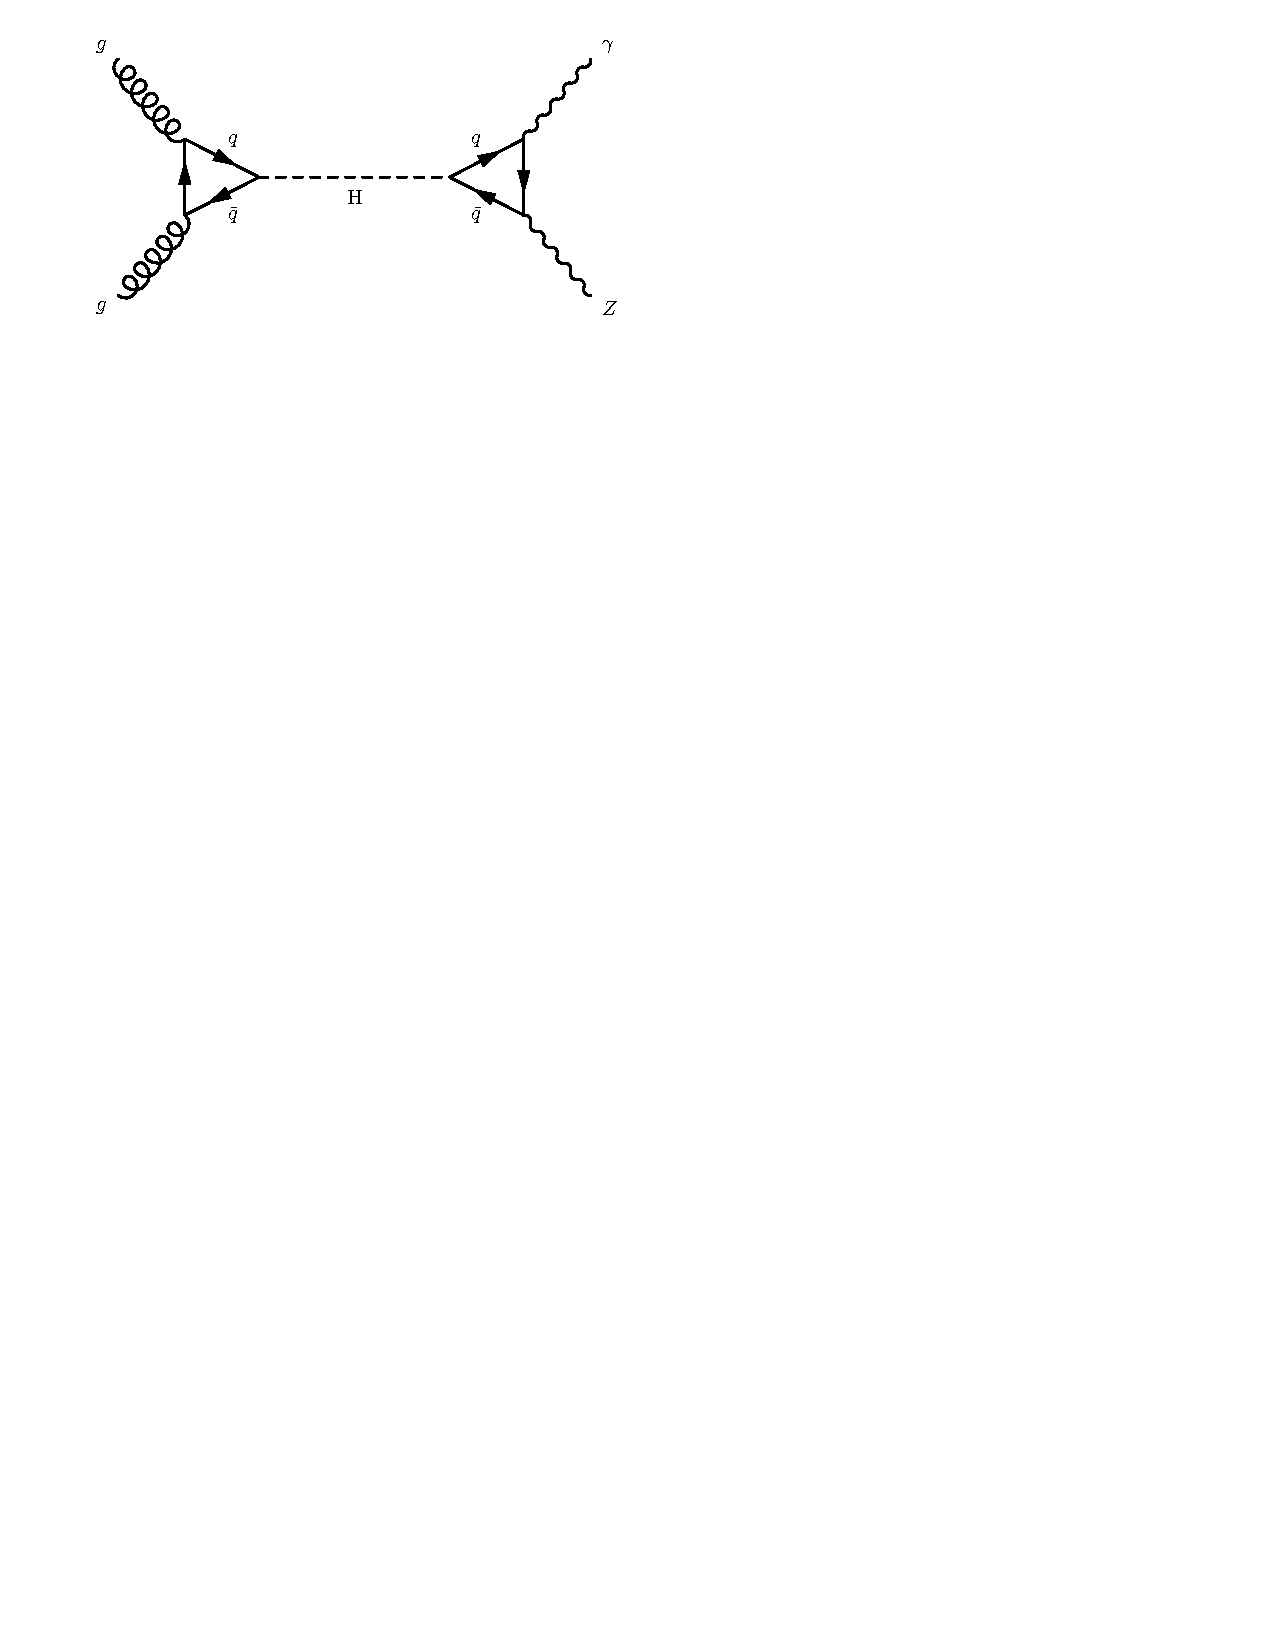
\includegraphics[trim={0.5cm 22cm 10cm 0cm},width=\textwidth]{../Diagrams/D17.pdf}
    \caption{$gg \rightarrow H \rightarrow Z\gamma$ (SI, WI, EM)}
    \label{fey:17}
  \end{subfigure}%
  ~
  \begin{subfigure}[b]{0.3\textwidth}
    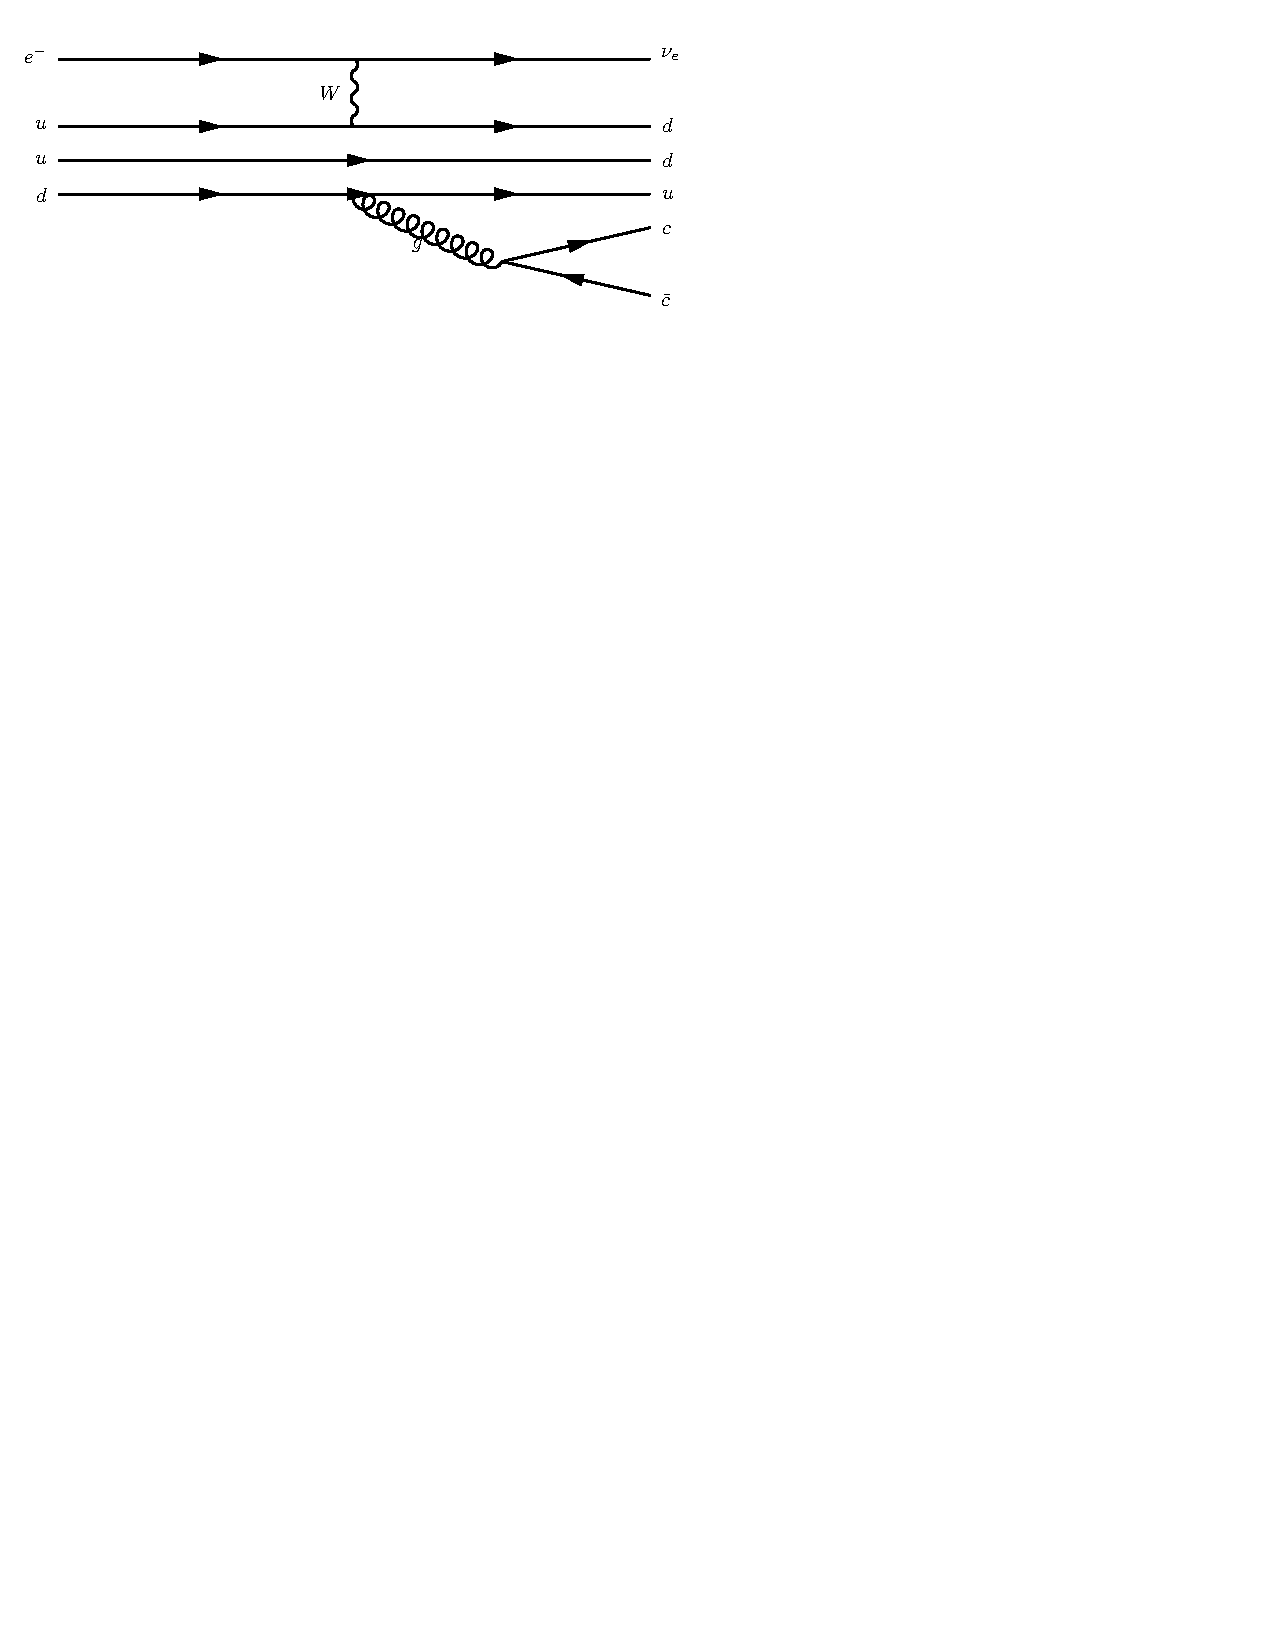
\includegraphics[trim={0.5cm 22cm 10cm 0cm},width=\textwidth]{../Diagrams/D18.pdf}
    \caption{$ep\rightarrow n\nu_eJ/\Psi$ (WI, SI)}
    \label{fey:18}
  \end{subfigure}%
\end{figure}

%\restoregeometry

\subsection{Suppression and forbidding of processes}
All the processes are fine when considering conservation numbers (with the possible exception of 5, explained below) such as family numbers, charge and spin. However, there are some processes that are unfavourable due to other phenomenon.

In process 5, it is suggested a anti-electron neutrino is created. This would violate lepton family number conservation, which is normally conserved, with the exception of neutrino oscillations. While it is a bit odd, the reaction is allowed, after some time. Momentarily after the reaction, however, there would have had to be a anti-muon neutrino, should the theoretical model be correct.

Process 9 show double Higgs production in an electron-positron annihilation. This brings about a problem due to the enormous difference in initial and final mass. When an electron is 

\section{\underline{Top quark and W-boson}}
\subsection{The CKM matrix and the function of the W-boson}
The Cabibbo-Kobayashi-Maskawa (CKM) matrix is defined as:

%see http://www.slac.stanford.edu/econf/C030626/bookpages/page142-152.pdf

\begin{equation}
\begin{bmatrix}
d' \\ s' \\ b'
\end{bmatrix} =
\begin{bmatrix}
V_{ud} & V_{us} & V_{ub} \\
V_{cd} & V_{cs} & V_{cb} \\
V_{td} & V_{ts} & V_{tb}
\end{bmatrix}
\begin{bmatrix}
d \\ s \\ b
\end{bmatrix}
\label{CKM_matrix}
\end{equation}

The right quark states are mass-eigenstates, meaning they are written a basis which diagonalizes the mass-matrix term in the Lagrangian density function. The left, Cabbibo-rotated, quark states are what couple to up-type quarks. The matrix is given by the equation:

\begin{equation}
V = U_u^\dagger U_d
\end{equation}

where $U_u$ and $U_d$ are the necessary rotations of the quark triplets (u,c,t) and (d,s,b) such that the mass matrices in the Lagrangian are diagonalized:

\begin{equation}
u_L^i \:\rightarrow\: U_u^{ij} u_L^j \:\:,\:\:
d_L^i \:\rightarrow\: U_d^{ij} d_L^j
\end{equation}

It is interesting to note that the CKM matrix, from its definition is believed to be unitary, which, so far, fits quite well with experimental results. In other words, in theory the entire matrix could be found be knowing only a bit more than half the terms. In the weak interaction, quark flavour can interchange by transition between up and down type quarks. This interchange is only permissible due to the W-boson. Theoretically, the W-boson links three $u_L^i$ fermion fields (quarks)\footnote{Here $L$ symbolizes the quarks being left-handed (doublets in $SU(2)$ representation), while the index $i$ is for each up quark flavour (u,c,t).} to the down type triplet. This can be seen from the equation:

\begin{equation}
J^{\mu+} = \frac{1}{\sqrt{2}}\bar{u}_L^i\gamma^\mu d_L^i \:\rightarrow\: \frac{1}{\sqrt{2}}\bar{u}_L^i\gamma^\mu (U_u^\dagger U_d)^{ij}d_L^j = 
\frac{1}{\sqrt{2}}\bar{u}_L^i\gamma^\mu V^{ij}d_L^j
\end{equation}

while quite out of context, this expression shows the transformation properties, under the rotation of mass eigenstates, of the terms in the Lagrangian that couple to the W-boson, where $J^{\mu+}$ (called the W-boson current) is the "coefficient" of the W-boson gauge field in the Lagrangian. As one sees, the W-boson only couples to one up-type and one down-type quark, meaning it's necessary for flavour changes in the weak interaction.\\

The elements of the CKM matrix can be determined experimentally, as the absolute squares of the elements are included in the coupling coefficients, and thus proportional to the branching ratio, which can be determined experimentally. Three of the elements have been determined using the following decays:

\begin{itemize}\centering
	\item Superallowed $\beta$-decay.
	\item $\text{K}^+ \:\rightarrow\: \pi^0\text{e}^+\nu_e$\\
	\item $\text{B}^0 \:\rightarrow\: \pi-\text{e}^+\nu_e$
\end{itemize}

How one can determine the matrix elements due to experimental data is because of the relation:

\begin{equation}
W_{i\rightarrow j} = \frac{BR(i \:\rightarrow\: j)}{\tau} \propto |V_{ij}|^2
\end{equation}

So by measuring the branching ratio of some decay, one can, by also knowing the decaying particle's average lifetime and the proportionality constant (determined theoretically or as form factors), solve for the absolute square of the matrix element. In case of the processes above, it was found (respectively):

\begin{itemize}\centering
	\item $|V_{ud}| = $
	\item $|V_{us}| = $
	\item $|V_{cb}| = $
\end{itemize}

\subsection{Top quark production}
There are 3 processes that are commonly used for top quark production: $\text{e}^-\text{e}^+$, $\text{p}\text{p}$ and $\text{p}\bar{\text{p}}$.\\
Electron-positron annihilation creates an intermediate photon or Z-boson that both can decay into a $l^-l^+$ state or $\text{q}\bar{\text{q}}$ state. Therefore, the process $\text{e}^-\text{e}^+ \:\rightarrow\: \text{t}\bar{\text{t}}$ is fully possible, if not a bit unfavourable. As there are two top quarks, there will be two jets, as a result of top-quark decay.\\
In a pp collision there are no annihilations, only high energy collisions. In these collisions, gluons are emitted from one or several of the quarks in one or both of the protons. It is therefore fairly straight forward to realise any one of these gluons can produce a top-anti-top product. With a bit of luck, many top-anti-top pairs can form, resulting in some even number of jets.\\
The final process, $\text{p}\bar{\text{p}}$, a quark and an anti-quark (either up or down) can annihilate to make a gluon which again makes a top-anti-top product.\\
The only two observed processes that produce a single top quark are:

\begin{itemize}
	\item $\text{W}^+\:\rightarrow\:\text{t}\bar{\text{b}}$
	\item $\text{b}\:\rightarrow\text{W}^-\text{t}$
\end{itemize}

The production of a $\text{W}^+$-boson can happen in a great number of ways in the process above, as any up-type quark can change type by emitting such a boson. The same can be said for a bottom quark, as a gluon can also decay into bottom-anti-bottom, either of which can decay into a top-flavour quark.

\subsection{Top quark decay}
The top quark decays by transforming into either a b,s or d quark, while emitting a W-boson. Of the three, it is far more likely to decay to a bottom quark, with a branching ratio of about 0.91. Considering this, it can decay in a limited number of ways, all of which are dependant on what the emitted W-boson decays into afterwards. Many usually just write the top-decay as $\text{t} \:\rightarrow\: \text{W}^+\text{b}$, without filling in the decay products of $\text{W}^+$.\\

Experimentally, the top quark 

\subsection{Branching ratios of two top quark decays}
The two top quark decays $t\:\rightarrow\text{b}+\text{c}\bar{\text{s}}$ and $t\:\rightarrow\text{b}+\tau+\nu_\tau$ occur by emission of a W-boson. As the top quark decays by weak interaction in both cases, the Sargent rule can be used to estimate the branching ratio of each process:

\begin{equation}
W_i = \frac{\Gamma_i/\Gamma}{\tau} \approx G_F^2 (\Delta m)^5
\end{equation}

where:

\begin{itemize}
	\item $W_i$ is the transition probability of decay process $i$.
	\item $\frac{\Gamma_i}{\Gamma}$ is the branching ratio of process $i$.
	\item $\tau$ is the average lifetime of the decaying particle. ($\tau \approx 5\times10^{-25}\text{s}$)
	\item $G_F = 1.1663787(6)\times 10^{-5}(\hbar c)^3\:\text{GeV}^{-2}$ is the Fermi constant.
	\item $\Delta m = m_i - \sum m_f$ is the difference in initial and final mass.
\end{itemize}

Furthermore, the particle masses needed are $m_t \approx 173.21\:\text{GeV}$, $m_b \approx 4.18\:\text{GeV}$, $m_s \approx 95 \pm 5 \:\text{MeV}$, $m_c \approx 1.275\:\text{GeV}$ and $m_\tau \approx 1776.8\:\text{MeV}$.\\
The only relevant difference between the two decays is the difference in final mass, which are $\Delta m \simeq m_t - m_b - m_\tau \simeq 167.25\:\text{GeV}$ and $\Delta m \simeq m_t - m_b - m_c - m_s \simeq 167.65\:\text{GeV}$.

\section{\underline{Gauge theories}}
\subsection{Symmetries and conservation laws of the standard model}
The standard model contains, among several, all the symmetries presented by the following direct product of groups:

\begin{equation}
	SU(3) \times SU(2) \times U(1)
\end{equation}

The product $SU(2) \times U(1)$ describes the electroweak theory; the unification of quantum electrodynamics (QED) and weak interaction (WI) theory (GWS theory\footnote{Sheldon Glashow, Abdus Salam and Steven Weinberg.}). It is also common to write $SU(2)_L$ to remind that the gauge fields of this group only couple to left-handed fermion fields.\\

Starting with the simplest, the symmetry group $U(1)$ is used in QED as one claims a local symmetry under unitary rotations of fermion fields (phase transform), i.e. the Lagrangian is invariant under:

\begin{equation}
	\psi \:\rightarrow\: e^{i\theta(x)}\psi
\end{equation} 

In order for this to hold, the covariant derivative must be introduced: $\bar{\psi}\slashed\partial\psi \:\rightarrow\: \bar{\psi}\slashed D\psi$. The covariant derivative ($D$) introduces a massless gauge field (usually denoted $A_\mu$), which behaves just like the photon as a force mediator.\\

The WI symmetry group has 3 generators (degrees of freedom for $SU(n):\:n^2-1$), which means there are 3 gauge bosons present in the covariant derivative. These gauge bosons can be used to make $\text{W}^\pm$ and $\text{W}^0$. Only with electroweak theory will one get $\text{Z}_ 0$. Invariance under $SU(2)_L$, where $L$ means the gauge fields only couple to left-handed fermion fields, can, in electroweak theory, be shown to conserve the weak isospin.\\

The QCD symmetry group has 8 generators (giving 8 gauge fields), which gives rise to 8 intermediate vector bosons (the gluons). In much the same manner as for WI, it can shown colour charge is conserved.

\subsection{The gauge principle and deriving the QCD Lagrangian}
The gauge principle is a procedure for finding how particles interact under certain continuous symmetries, which in the case of the standard model are under $SU(3)$, $SU(2)$ and $U(1)$\footnote{There are other symmetries in the Standard model, but none that provide insight to interactions, e.g. Lorentz invariance.}. By starting with the free field Lagrangian, it is demanded the Dirac field is invariant under some local\footnote{By locality, one means a continuous transform under the symmetry group at some space-time point. The physical reason for such a demand is that ...} symmetry transformation. In order to fulfil such a demand, certain changes to the Lagrangian must be done (making a covariant derivative), which is the where the exchange bosons come into play.\\

The $SU(3)$ symmetry group and it's role in the standard model came about not long after the propositions of the "eightfold way", to categorize baryons according to their quantum numbers, and quark flavour to explain the these numbers (isospin, ).\\
However, this did not explain the existence of the $\Omega^-$ hyperon, which seemed to violate the Pauli exclusion principle due to its constituents all, apparently, existing in the same state. Therefore, the colour charge was proposed; each baryons' quarks had a different colour charge, so there were 3 possible "colours". This is why the irreducible representation of $SU(3)$ fits nicely in with its three degrees of freedom and where quantum chromodynamics has its birth.\\

Deriving the QCD Lagrangian by the gauge principle is done as follows; starting with the free Lagrangian

\begin{equation}
	\mathcal{L}_{free} = \sum_f \bar{q}_f\left(i\slashed \partial - m_f\right)q_f
\end{equation}

where $q_f$ is a Dirac spinor for flavour type $f$, a $SU(3)$ field transformation is performed:

\begin{equation}
	q_f^\alpha \:\rightarrow\: U^\alpha_\beta q_f^\beta
\end{equation} 

where $U = e^{-ig_s\frac{\lambda^a}{2}\theta_a}$ and $\lambda^a$ are the Gellmann matrices in the fundamental representation. As is standard, now locality is demanded: $\theta_a \:\rightarrow\: \theta_a(x)$. Of course, the problem now is that the Lagrangian is not invariant under such a transform, so a covariant derivative must be found.\\
In non-abelian gauge theory, for local invariance under some symmetry (Lie) group ($\psi \:\rightarrow\: V(x)\psi$), The unitary matrix $V(x)$ can be expanded infinitesimally about $x$:

\begin{equation}
	V(x) = 1 + i\alpha^i(x)t^a + \mathcal{O}(\alpha^2)
\end{equation}

where $t^a$ are the generators of the group and $\alpha^i$ some rotation. From the definition of the covariant derivative along a vector $n^\mu$:

\begin{equation}
	n^\mu D_\mu\psi = \lim_{\epsilon\:\rightarrow\:0} \frac{1}{\epsilon}\left[\psi(x+\epsilon x) - U(x+\epsilon x,x)\psi(x)\right]
	\label{Def_of_D}
\end{equation}

where

\begin{equation}
	U(y,x) \:\rightarrow\: V(y)U(y,x)V^\dagger(x)
\end{equation}

So by infinitesimal expansion, in the case of $SU(3)$ ($V(x) = e^{-ig_s\frac{\lambda^a}{2}\theta_a(x)}$):

\begin{equation}
	U(x+\epsilon, x) = 1 + ig_s\epsilon n^\mu G_\mu^a \lambda_a + \mathcal{O}(\epsilon^2)
\end{equation}

Here $G_\mu^a$ are the gauge fields of $SU(3)$, later to be identified with the gluon fields. The absence of $\theta$, from $V$, is due to the details of the expansion. When inserting the above in equation \ref{Def_of_D} and taking the limit, it follows:

\begin{equation}
	D^\mu q_f = \left[ \partial^\mu - ig_s\frac{\lambda^a}{2}G_a^\mu(x) \right]q_f
\end{equation}

In order for this to transform in the same manner as the quark field alone,

Thus the first order interactive term between the quarks and gluons is found, but the gauge-invariant kinetic gluon term remains hidden. Again, from non-abelian gauge theory it is known that the field strength must be found. To find it, it is necessary\footnote{At least by approaching the problem with infinitesimal expansion.} to know the transformation properties of $q_f^a$ and $G_a^\mu$ separately:

\begin{align}
	q_f^a &\:\rightarrow\: q_f^a - ig_s\left(\frac{\lambda^a}{2}\right)_{\alpha\beta}\\
	&=
\end{align}



\end{document}